% Options for packages loaded elsewhere
\PassOptionsToPackage{unicode}{hyperref}
\PassOptionsToPackage{hyphens}{url}
%
\documentclass[
]{article}
\usepackage{amsmath,amssymb}
\usepackage{iftex}
\ifPDFTeX
  \usepackage[T1]{fontenc}
  \usepackage[utf8]{inputenc}
  \usepackage{textcomp} % provide euro and other symbols
\else % if luatex or xetex
  \usepackage{unicode-math} % this also loads fontspec
  \defaultfontfeatures{Scale=MatchLowercase}
  \defaultfontfeatures[\rmfamily]{Ligatures=TeX,Scale=1}
\fi
\usepackage{lmodern}
\ifPDFTeX\else
  % xetex/luatex font selection
\fi
% Use upquote if available, for straight quotes in verbatim environments
\IfFileExists{upquote.sty}{\usepackage{upquote}}{}
\IfFileExists{microtype.sty}{% use microtype if available
  \usepackage[]{microtype}
  \UseMicrotypeSet[protrusion]{basicmath} % disable protrusion for tt fonts
}{}
\makeatletter
\@ifundefined{KOMAClassName}{% if non-KOMA class
  \IfFileExists{parskip.sty}{%
    \usepackage{parskip}
  }{% else
    \setlength{\parindent}{0pt}
    \setlength{\parskip}{6pt plus 2pt minus 1pt}}
}{% if KOMA class
  \KOMAoptions{parskip=half}}
\makeatother
\usepackage{xcolor}
\usepackage[margin=1in]{geometry}
\usepackage{color}
\usepackage{fancyvrb}
\newcommand{\VerbBar}{|}
\newcommand{\VERB}{\Verb[commandchars=\\\{\}]}
\DefineVerbatimEnvironment{Highlighting}{Verbatim}{commandchars=\\\{\}}
% Add ',fontsize=\small' for more characters per line
\usepackage{framed}
\definecolor{shadecolor}{RGB}{248,248,248}
\newenvironment{Shaded}{\begin{snugshade}}{\end{snugshade}}
\newcommand{\AlertTok}[1]{\textcolor[rgb]{0.94,0.16,0.16}{#1}}
\newcommand{\AnnotationTok}[1]{\textcolor[rgb]{0.56,0.35,0.01}{\textbf{\textit{#1}}}}
\newcommand{\AttributeTok}[1]{\textcolor[rgb]{0.13,0.29,0.53}{#1}}
\newcommand{\BaseNTok}[1]{\textcolor[rgb]{0.00,0.00,0.81}{#1}}
\newcommand{\BuiltInTok}[1]{#1}
\newcommand{\CharTok}[1]{\textcolor[rgb]{0.31,0.60,0.02}{#1}}
\newcommand{\CommentTok}[1]{\textcolor[rgb]{0.56,0.35,0.01}{\textit{#1}}}
\newcommand{\CommentVarTok}[1]{\textcolor[rgb]{0.56,0.35,0.01}{\textbf{\textit{#1}}}}
\newcommand{\ConstantTok}[1]{\textcolor[rgb]{0.56,0.35,0.01}{#1}}
\newcommand{\ControlFlowTok}[1]{\textcolor[rgb]{0.13,0.29,0.53}{\textbf{#1}}}
\newcommand{\DataTypeTok}[1]{\textcolor[rgb]{0.13,0.29,0.53}{#1}}
\newcommand{\DecValTok}[1]{\textcolor[rgb]{0.00,0.00,0.81}{#1}}
\newcommand{\DocumentationTok}[1]{\textcolor[rgb]{0.56,0.35,0.01}{\textbf{\textit{#1}}}}
\newcommand{\ErrorTok}[1]{\textcolor[rgb]{0.64,0.00,0.00}{\textbf{#1}}}
\newcommand{\ExtensionTok}[1]{#1}
\newcommand{\FloatTok}[1]{\textcolor[rgb]{0.00,0.00,0.81}{#1}}
\newcommand{\FunctionTok}[1]{\textcolor[rgb]{0.13,0.29,0.53}{\textbf{#1}}}
\newcommand{\ImportTok}[1]{#1}
\newcommand{\InformationTok}[1]{\textcolor[rgb]{0.56,0.35,0.01}{\textbf{\textit{#1}}}}
\newcommand{\KeywordTok}[1]{\textcolor[rgb]{0.13,0.29,0.53}{\textbf{#1}}}
\newcommand{\NormalTok}[1]{#1}
\newcommand{\OperatorTok}[1]{\textcolor[rgb]{0.81,0.36,0.00}{\textbf{#1}}}
\newcommand{\OtherTok}[1]{\textcolor[rgb]{0.56,0.35,0.01}{#1}}
\newcommand{\PreprocessorTok}[1]{\textcolor[rgb]{0.56,0.35,0.01}{\textit{#1}}}
\newcommand{\RegionMarkerTok}[1]{#1}
\newcommand{\SpecialCharTok}[1]{\textcolor[rgb]{0.81,0.36,0.00}{\textbf{#1}}}
\newcommand{\SpecialStringTok}[1]{\textcolor[rgb]{0.31,0.60,0.02}{#1}}
\newcommand{\StringTok}[1]{\textcolor[rgb]{0.31,0.60,0.02}{#1}}
\newcommand{\VariableTok}[1]{\textcolor[rgb]{0.00,0.00,0.00}{#1}}
\newcommand{\VerbatimStringTok}[1]{\textcolor[rgb]{0.31,0.60,0.02}{#1}}
\newcommand{\WarningTok}[1]{\textcolor[rgb]{0.56,0.35,0.01}{\textbf{\textit{#1}}}}
\usepackage{graphicx}
\makeatletter
\def\maxwidth{\ifdim\Gin@nat@width>\linewidth\linewidth\else\Gin@nat@width\fi}
\def\maxheight{\ifdim\Gin@nat@height>\textheight\textheight\else\Gin@nat@height\fi}
\makeatother
% Scale images if necessary, so that they will not overflow the page
% margins by default, and it is still possible to overwrite the defaults
% using explicit options in \includegraphics[width, height, ...]{}
\setkeys{Gin}{width=\maxwidth,height=\maxheight,keepaspectratio}
% Set default figure placement to htbp
\makeatletter
\def\fps@figure{htbp}
\makeatother
\setlength{\emergencystretch}{3em} % prevent overfull lines
\providecommand{\tightlist}{%
  \setlength{\itemsep}{0pt}\setlength{\parskip}{0pt}}
\setcounter{secnumdepth}{-\maxdimen} % remove section numbering
\ifLuaTeX
  \usepackage{selnolig}  % disable illegal ligatures
\fi
\usepackage{bookmark}
\IfFileExists{xurl.sty}{\usepackage{xurl}}{} % add URL line breaks if available
\urlstyle{same}
\hypersetup{
  pdftitle={Figures\_FLUXNET},
  hidelinks,
  pdfcreator={LaTeX via pandoc}}

\title{Figures\_FLUXNET}
\author{}
\date{\vspace{-2.5em}2025-04-23}

\begin{document}
\maketitle

\section{FLUXNET data}\label{fluxnet-data}

\begin{itemize}
\tightlist
\item
  variables quick start guide
  \url{https://fluxnet.org/data/fluxnet2015-dataset/variables-quick-start-guide/}
\item
  data variables:
  \url{https://fluxnet.org/data/aboutdata/data-variables/}
\item
  full set data product:
  \url{https://fluxnet.org/data/fluxnet2015-dataset/fullset-data-product/}
\end{itemize}

\section{Working on annual data (YY)}\label{working-on-annual-data-yy}

\subsection{read in data}\label{read-in-data}

\begin{Shaded}
\begin{Highlighting}[]
\NormalTok{filename }\OtherTok{=} \StringTok{"AMF\_US{-}Syv\_FLUXNET\_SUBSET\_YY\_2001{-}2023\_4{-}6.csv"}
\FunctionTok{setwd}\NormalTok{(data\_dir); df.YY }\OtherTok{=} \FunctionTok{fread}\NormalTok{(filename)}
\NormalTok{df.YY}\SpecialCharTok{$}\NormalTok{year }\OtherTok{=} \FunctionTok{as.numeric}\NormalTok{(df.YY}\SpecialCharTok{$}\NormalTok{TIMESTAMP)}
\NormalTok{df.YY }\OtherTok{\textless{}{-}}\NormalTok{ df.YY }\SpecialCharTok{\%\textgreater{}\%}
  \FunctionTok{mutate}\NormalTok{(}\FunctionTok{across}\NormalTok{(}\FunctionTok{everything}\NormalTok{(), }\SpecialCharTok{\textasciitilde{}}\FunctionTok{na\_if}\NormalTok{(. , }\SpecialCharTok{{-}}\DecValTok{9999}\NormalTok{)))}
\end{Highlighting}
\end{Shaded}

\subsection{Figure 1: annual sums of
NEE}\label{figure-1-annual-sums-of-nee}

Variables expressing random uncertainty are identified by the suffix
\_RANDUNC. One of two methods are used to estimate random uncertainty,
applied hierarchically: - NEE-RANDUNC Method 1 (direct standard
deviation method) - NEE-RANDUNC Method 2 (median standard deviation
method) - For more details, please check out Pastorello et al.~2020

\begin{Shaded}
\begin{Highlighting}[]
\CommentTok{\# create upper and lower bounds}
\CommentTok{\# NEE\_VUT\_REF\_RANDUNC}
\NormalTok{df.YY}\SpecialCharTok{$}\NormalTok{NEE\_upper }\OtherTok{\textless{}{-}}\NormalTok{ df.YY}\SpecialCharTok{$}\NormalTok{NEE\_VUT\_REF }\SpecialCharTok{+}\NormalTok{ df.YY}\SpecialCharTok{$}\NormalTok{NEE\_VUT\_REF\_RANDUNC}
\NormalTok{df.YY}\SpecialCharTok{$}\NormalTok{NEE\_lower }\OtherTok{\textless{}{-}}\NormalTok{ df.YY}\SpecialCharTok{$}\NormalTok{NEE\_VUT\_REF }\SpecialCharTok{{-}}\NormalTok{ df.YY}\SpecialCharTok{$}\NormalTok{NEE\_VUT\_REF\_RANDUNC}

\CommentTok{\# plot annual sums of NEE across years}
\FunctionTok{ggplot}\NormalTok{(df.YY, }\FunctionTok{aes}\NormalTok{(}\AttributeTok{x =}\NormalTok{ year)) }\SpecialCharTok{+}
  \FunctionTok{geom\_ribbon}\NormalTok{(}\FunctionTok{aes}\NormalTok{(}\AttributeTok{ymin =}\NormalTok{ NEE\_lower, }\AttributeTok{ymax =}\NormalTok{ NEE\_upper), }\AttributeTok{fill =} \StringTok{"blue"}\NormalTok{, }\AttributeTok{alpha =} \FloatTok{0.4}\NormalTok{) }\SpecialCharTok{+} \CommentTok{\# random uncertainty }
  \FunctionTok{geom\_line}\NormalTok{(}\FunctionTok{aes}\NormalTok{(}\AttributeTok{y =}\NormalTok{ NEE\_VUT\_REF), }\AttributeTok{color =} \StringTok{"black"}\NormalTok{, }\AttributeTok{size =} \DecValTok{1}\NormalTok{) }\SpecialCharTok{+}
  \FunctionTok{geom\_smooth}\NormalTok{(}\FunctionTok{aes}\NormalTok{(}\AttributeTok{y =}\NormalTok{ NEE\_VUT\_REF), }\AttributeTok{method =} \StringTok{"lm"}\NormalTok{, }\AttributeTok{color =} \StringTok{"red"}\NormalTok{, }\AttributeTok{se =} \ConstantTok{FALSE}\NormalTok{, }\AttributeTok{linetype =} \StringTok{"dashed"}\NormalTok{) }\SpecialCharTok{+} \CommentTok{\# Trend line}
  \FunctionTok{ggtitle}\NormalTok{(}\StringTok{"Annual sums of NEE"}\NormalTok{) }\SpecialCharTok{+}\NormalTok{ my\_theme}
\end{Highlighting}
\end{Shaded}

\includegraphics{FLUXNET_files/figure-latex/unnamed-chunk-2-1.pdf}

\begin{Shaded}
\begin{Highlighting}[]
\CommentTok{\# The Mann{-}Kendall trend test is used to assess whether there is a significant monotonic trend (either increasing or decreasing) in a time series. }
\FunctionTok{MannKendall}\NormalTok{(df.YY}\SpecialCharTok{$}\NormalTok{NEE\_VUT\_REF) }\CommentTok{\# When P \textless{} 0.05, you can reject the null hypothesis ("no trend").}
\end{Highlighting}
\end{Shaded}

\begin{verbatim}
## tau = -0.228, 2-sided pvalue =0.1837
\end{verbatim}

\begin{Shaded}
\begin{Highlighting}[]
\CommentTok{\# plot qualify flags of NEE}
\FunctionTok{ggplot}\NormalTok{(df.YY, }\FunctionTok{aes}\NormalTok{(}\AttributeTok{x =} \FunctionTok{as.factor}\NormalTok{(year), }\AttributeTok{y =}\NormalTok{ NEE\_VUT\_REF\_QC)) }\SpecialCharTok{+}
  \FunctionTok{geom\_bar}\NormalTok{(}\AttributeTok{stat =} \StringTok{"identity"}\NormalTok{, }\AttributeTok{fill =} \StringTok{"grey"}\NormalTok{) }\SpecialCharTok{+}
  \FunctionTok{geom\_hline}\NormalTok{(}\AttributeTok{yintercept =} \FloatTok{0.75}\NormalTok{, }\AttributeTok{linetype =} \StringTok{"dashed"}\NormalTok{, }\AttributeTok{color =} \StringTok{"red"}\NormalTok{) }\SpecialCharTok{+}
  \FunctionTok{labs}\NormalTok{(}\AttributeTok{x =} \StringTok{"Year"}\NormalTok{, }\AttributeTok{y =} \StringTok{"NEE\_VUT\_REF\_QC"}\NormalTok{, }\AttributeTok{title =} \StringTok{"Qualify flags for annual sums"}\NormalTok{) }\SpecialCharTok{+}
  \FunctionTok{ylim}\NormalTok{(}\DecValTok{0}\NormalTok{,}\DecValTok{1}\NormalTok{) }\SpecialCharTok{+}\NormalTok{  my\_theme}
\end{Highlighting}
\end{Shaded}

\includegraphics{FLUXNET_files/figure-latex/unnamed-chunk-2-2.pdf}

Where to go from here: - Interpret the figure and include it in your
group presentation. - Plot annual sums (uncertainty) of LE and H. -
Explore the qualify flags for annual sums of LE and H.

\section{Working with half hourly data
(HH)}\label{working-with-half-hourly-data-hh}

\subsection{read in half hourly data}\label{read-in-half-hourly-data}

\begin{Shaded}
\begin{Highlighting}[]
\FunctionTok{setwd}\NormalTok{(data\_dir); df.HH }\OtherTok{=} \FunctionTok{fread}\NormalTok{(}\FunctionTok{paste0}\NormalTok{(}\StringTok{"AMF\_US{-}Syv\_FLUXNET\_SUBSET\_HH\_2001{-}2023\_4{-}6.csv"}\NormalTok{)) }
\CommentTok{\# FLUXNET data uses "{-}9999" as placeholder for missing data. Replace {-}9999 with NA across all columns}
\NormalTok{df.HH }\OtherTok{\textless{}{-}}\NormalTok{ df.HH }\SpecialCharTok{\%\textgreater{}\%}
  \FunctionTok{mutate}\NormalTok{(}\FunctionTok{across}\NormalTok{(}\FunctionTok{everything}\NormalTok{(), }\SpecialCharTok{\textasciitilde{}}\FunctionTok{na\_if}\NormalTok{(. , }\SpecialCharTok{{-}}\DecValTok{9999}\NormalTok{)))}

\CommentTok{\# Timestamp column of flux data is formatted as YYYYMMDDHHMM. We need to change it to a readable timestamp format.}
\FunctionTok{class}\NormalTok{(df.HH}\SpecialCharTok{$}\NormalTok{TIMESTAMP\_END)}
\end{Highlighting}
\end{Shaded}

\begin{verbatim}
## [1] "integer64"
\end{verbatim}

\begin{Shaded}
\begin{Highlighting}[]
\NormalTok{df.HH}\SpecialCharTok{$}\NormalTok{TIMESTAMP\_END }\OtherTok{\textless{}{-}} \FunctionTok{ymd\_hm}\NormalTok{(}\FunctionTok{as.character}\NormalTok{(df.HH}\SpecialCharTok{$}\NormalTok{TIMESTAMP\_END))}
\FunctionTok{class}\NormalTok{(df.HH}\SpecialCharTok{$}\NormalTok{TIMESTAMP\_END)}
\end{Highlighting}
\end{Shaded}

\begin{verbatim}
## [1] "POSIXct" "POSIXt"
\end{verbatim}

\begin{Shaded}
\begin{Highlighting}[]
\CommentTok{\# Create columns of year and month}
\NormalTok{df.HH }\OtherTok{\textless{}{-}}\NormalTok{ df.HH }\SpecialCharTok{\%\textgreater{}\%}
  \FunctionTok{mutate}\NormalTok{(}\AttributeTok{year =} \FunctionTok{year}\NormalTok{(TIMESTAMP\_END), }\AttributeTok{month =} \FunctionTok{month}\NormalTok{(TIMESTAMP\_END))}
\end{Highlighting}
\end{Shaded}

\subsection{Figure 2: qualify flags of half-hourly
data}\label{figure-2-qualify-flags-of-half-hourly-data}

\begin{Shaded}
\begin{Highlighting}[]
\NormalTok{df.HH }\OtherTok{\textless{}{-}}\NormalTok{ df.HH }\SpecialCharTok{\%\textgreater{}\%} \CommentTok{\# using half{-}hourly data}
  \FunctionTok{mutate}\NormalTok{(}
    \AttributeTok{year =} \FunctionTok{year}\NormalTok{(TIMESTAMP\_END),}
    \AttributeTok{DOY =} \FunctionTok{yday}\NormalTok{(TIMESTAMP\_END) }\SpecialCharTok{+} 
\NormalTok{      (}\FunctionTok{hour}\NormalTok{(TIMESTAMP\_END) }\SpecialCharTok{+} \FunctionTok{minute}\NormalTok{(TIMESTAMP\_END)}\SpecialCharTok{/}\DecValTok{60} \SpecialCharTok{+} \FunctionTok{second}\NormalTok{(TIMESTAMP\_END)}\SpecialCharTok{/}\DecValTok{3600}\NormalTok{) }\SpecialCharTok{/} \DecValTok{24}\NormalTok{,}
    \AttributeTok{qc\_label =} \FunctionTok{factor}\NormalTok{(}
\NormalTok{      NEE\_VUT\_REF\_QC,}
      \AttributeTok{levels =} \FunctionTok{c}\NormalTok{(}\DecValTok{0}\NormalTok{, }\DecValTok{1}\NormalTok{, }\DecValTok{2}\NormalTok{, }\DecValTok{3}\NormalTok{),}
      \AttributeTok{labels =} \FunctionTok{c}\NormalTok{(}\StringTok{"Measured (0)"}\NormalTok{, }\StringTok{"Good (1)"}\NormalTok{, }\StringTok{"Medium (2)"}\NormalTok{, }\StringTok{"Poor (3)"}\NormalTok{)}
\NormalTok{    )}
\NormalTok{  )}

\CommentTok{\#calculate the percentage of each flag}
\NormalTok{qc\_summary }\OtherTok{\textless{}{-}}\NormalTok{ df.HH }\SpecialCharTok{\%\textgreater{}\%}
  \FunctionTok{group\_by}\NormalTok{(year, qc\_label) }\SpecialCharTok{\%\textgreater{}\%}
  \FunctionTok{summarise}\NormalTok{(}\AttributeTok{count =} \FunctionTok{n}\NormalTok{(), }\AttributeTok{.groups =} \StringTok{"drop"}\NormalTok{) }\SpecialCharTok{\%\textgreater{}\%}
  \FunctionTok{group\_by}\NormalTok{(year) }\SpecialCharTok{\%\textgreater{}\%}
  \FunctionTok{mutate}\NormalTok{(}
    \AttributeTok{total =} \FunctionTok{sum}\NormalTok{(count),}
    \AttributeTok{percent =} \FunctionTok{round}\NormalTok{(}\DecValTok{100} \SpecialCharTok{*}\NormalTok{ count }\SpecialCharTok{/}\NormalTok{ total, }\DecValTok{1}\NormalTok{),}
    \AttributeTok{label =} \FunctionTok{paste0}\NormalTok{(qc\_label, }\StringTok{": "}\NormalTok{, percent, }\StringTok{"\%"}\NormalTok{)}
\NormalTok{  )}
\CommentTok{\# View(qc\_summary)}

\CommentTok{\# plot qc\_summary by year}
\NormalTok{qc\_summary }\SpecialCharTok{\%\textgreater{}\%}
  \FunctionTok{filter}\NormalTok{(year }\SpecialCharTok{\textgreater{}=} \DecValTok{2004}\NormalTok{, year }\SpecialCharTok{\textless{}=} \DecValTok{2022}\NormalTok{) }\SpecialCharTok{\%\textgreater{}\%}
  \FunctionTok{ggplot}\NormalTok{(}\FunctionTok{aes}\NormalTok{(}\AttributeTok{x =} \FunctionTok{factor}\NormalTok{(year), }\AttributeTok{y =}\NormalTok{ percent, }\AttributeTok{fill =}\NormalTok{ qc\_label)) }\SpecialCharTok{+}
  \FunctionTok{geom\_bar}\NormalTok{(}\AttributeTok{stat =} \StringTok{"identity"}\NormalTok{) }\SpecialCharTok{+}
  \FunctionTok{scale\_fill\_manual}\NormalTok{(}
    \AttributeTok{name =} \StringTok{"QC Flag"}\NormalTok{,}
    \AttributeTok{values =} \FunctionTok{c}\NormalTok{(}
      \StringTok{"Measured (0)"} \OtherTok{=} \StringTok{"black"}\NormalTok{,}
      \StringTok{"Good (1)"} \OtherTok{=} \StringTok{"green4"}\NormalTok{,}
      \StringTok{"Medium (2)"} \OtherTok{=} \StringTok{"orange"}\NormalTok{,}
      \StringTok{"Poor (3)"} \OtherTok{=} \StringTok{"red"}
\NormalTok{    )}
\NormalTok{  ) }\SpecialCharTok{+}
  \FunctionTok{labs}\NormalTok{(}
    \AttributeTok{title =} \StringTok{"Summary of NEE Quality Flags"}\NormalTok{,}
    \AttributeTok{x =} \StringTok{"Year"}\NormalTok{, }\AttributeTok{y =} \StringTok{"Percentage (\%)"}
\NormalTok{  ) }\SpecialCharTok{+}\NormalTok{ my\_theme}
\end{Highlighting}
\end{Shaded}

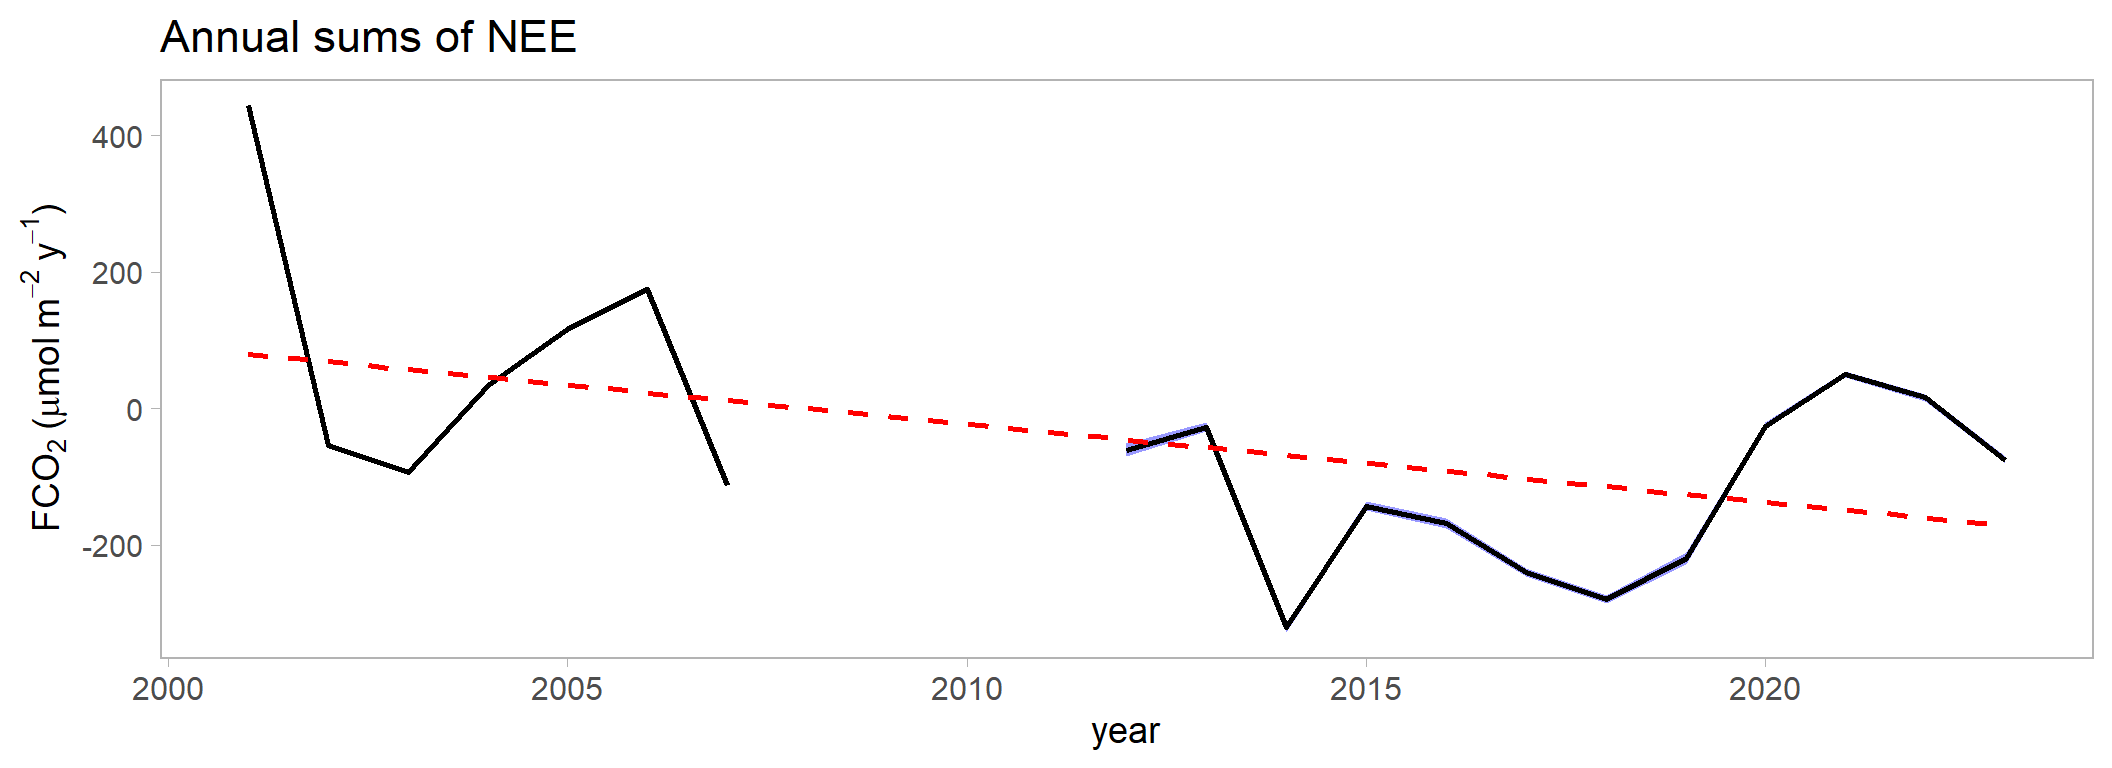
\includegraphics{FLUXNET_files/figure-latex/unnamed-chunk-4-1.pdf}

\begin{Shaded}
\begin{Highlighting}[]
\NormalTok{qc\_labels }\OtherTok{\textless{}{-}}\NormalTok{ qc\_summary }\SpecialCharTok{\%\textgreater{}\%}
  \FunctionTok{group\_by}\NormalTok{(year) }\SpecialCharTok{\%\textgreater{}\%}
  \FunctionTok{summarise}\NormalTok{(}
    \AttributeTok{qc\_text =} \FunctionTok{paste}\NormalTok{(label, }\AttributeTok{collapse =} \StringTok{"}\SpecialCharTok{\textbackslash{}n}\StringTok{"}\NormalTok{),}
    \AttributeTok{.groups =} \StringTok{"drop"}
\NormalTok{  )}

\NormalTok{data\_with\_labels }\OtherTok{\textless{}{-}}\NormalTok{ df.HH }\SpecialCharTok{\%\textgreater{}\%}
  \FunctionTok{left\_join}\NormalTok{(qc\_labels, }\AttributeTok{by =} \StringTok{"year"}\NormalTok{)}

\CommentTok{\# looking into data for one year: plot NEE with QC flags}
\NormalTok{data\_with\_labels }\SpecialCharTok{\%\textgreater{}\%}
  \FunctionTok{filter}\NormalTok{(year }\SpecialCharTok{==} \DecValTok{2018}\NormalTok{) }\SpecialCharTok{\%\textgreater{}\%} 
  \FunctionTok{ggplot}\NormalTok{(}\FunctionTok{aes}\NormalTok{(}\AttributeTok{x =}\NormalTok{ DOY, }\AttributeTok{y =}\NormalTok{ NEE\_VUT\_REF, }\AttributeTok{color =}\NormalTok{ qc\_label)) }\SpecialCharTok{+}
  \FunctionTok{geom\_point}\NormalTok{(}\AttributeTok{alpha =} \FloatTok{0.6}\NormalTok{, }\AttributeTok{size =} \DecValTok{1}\NormalTok{) }\SpecialCharTok{+}
  \FunctionTok{scale\_color\_manual}\NormalTok{(}
    \AttributeTok{name =} \StringTok{"QC Flag"}\NormalTok{,}
    \AttributeTok{values =} \FunctionTok{c}\NormalTok{(}\StringTok{"Measured (0)"} \OtherTok{=} \StringTok{"black"}\NormalTok{,}
               \StringTok{"Good (1)"} \OtherTok{=} \StringTok{"green4"}\NormalTok{,}
               \StringTok{"Medium (2)"} \OtherTok{=} \StringTok{"orange"}\NormalTok{,}
               \StringTok{"Poor (3)"} \OtherTok{=} \StringTok{"red"}\NormalTok{)}
\NormalTok{  ) }\SpecialCharTok{+}
  \FunctionTok{geom\_text}\NormalTok{(}
    \AttributeTok{data =}\NormalTok{ qc\_labels,}
    \FunctionTok{aes}\NormalTok{(}\AttributeTok{x =} \DecValTok{12}\NormalTok{, }\AttributeTok{y =} \DecValTok{20}\NormalTok{, }\AttributeTok{label =}\NormalTok{ qc\_text),}
    \AttributeTok{inherit.aes =} \ConstantTok{FALSE}\NormalTok{,}
    \AttributeTok{hjust =} \DecValTok{0}\NormalTok{,}
    \AttributeTok{vjust =} \FloatTok{1.1}\NormalTok{,}
    \AttributeTok{size =} \DecValTok{3}\NormalTok{,}
    \AttributeTok{color =} \StringTok{"gray30"}
\NormalTok{  ) }\SpecialCharTok{+}
  \FunctionTok{labs}\NormalTok{(}
    \AttributeTok{title =} \StringTok{"Half hourly FCO2 and quality flags for a single year"}\NormalTok{,}
    \AttributeTok{x =} \StringTok{"DOY"}\NormalTok{, }\AttributeTok{y =} \FunctionTok{expression}\NormalTok{(FCO2}\SpecialCharTok{\textasciitilde{}}\NormalTok{(g}\SpecialCharTok{\textasciitilde{}}\NormalTok{C}\SpecialCharTok{\textasciitilde{}}\NormalTok{m}\SpecialCharTok{\^{}}\NormalTok{\{}\SpecialCharTok{{-}}\DecValTok{2}\NormalTok{\}}\SpecialCharTok{\textasciitilde{}}\NormalTok{d}\SpecialCharTok{\^{}}\NormalTok{\{}\SpecialCharTok{{-}}\DecValTok{1}\NormalTok{\})) }
\NormalTok{  ) }\SpecialCharTok{+}\NormalTok{ my\_theme}
\end{Highlighting}
\end{Shaded}

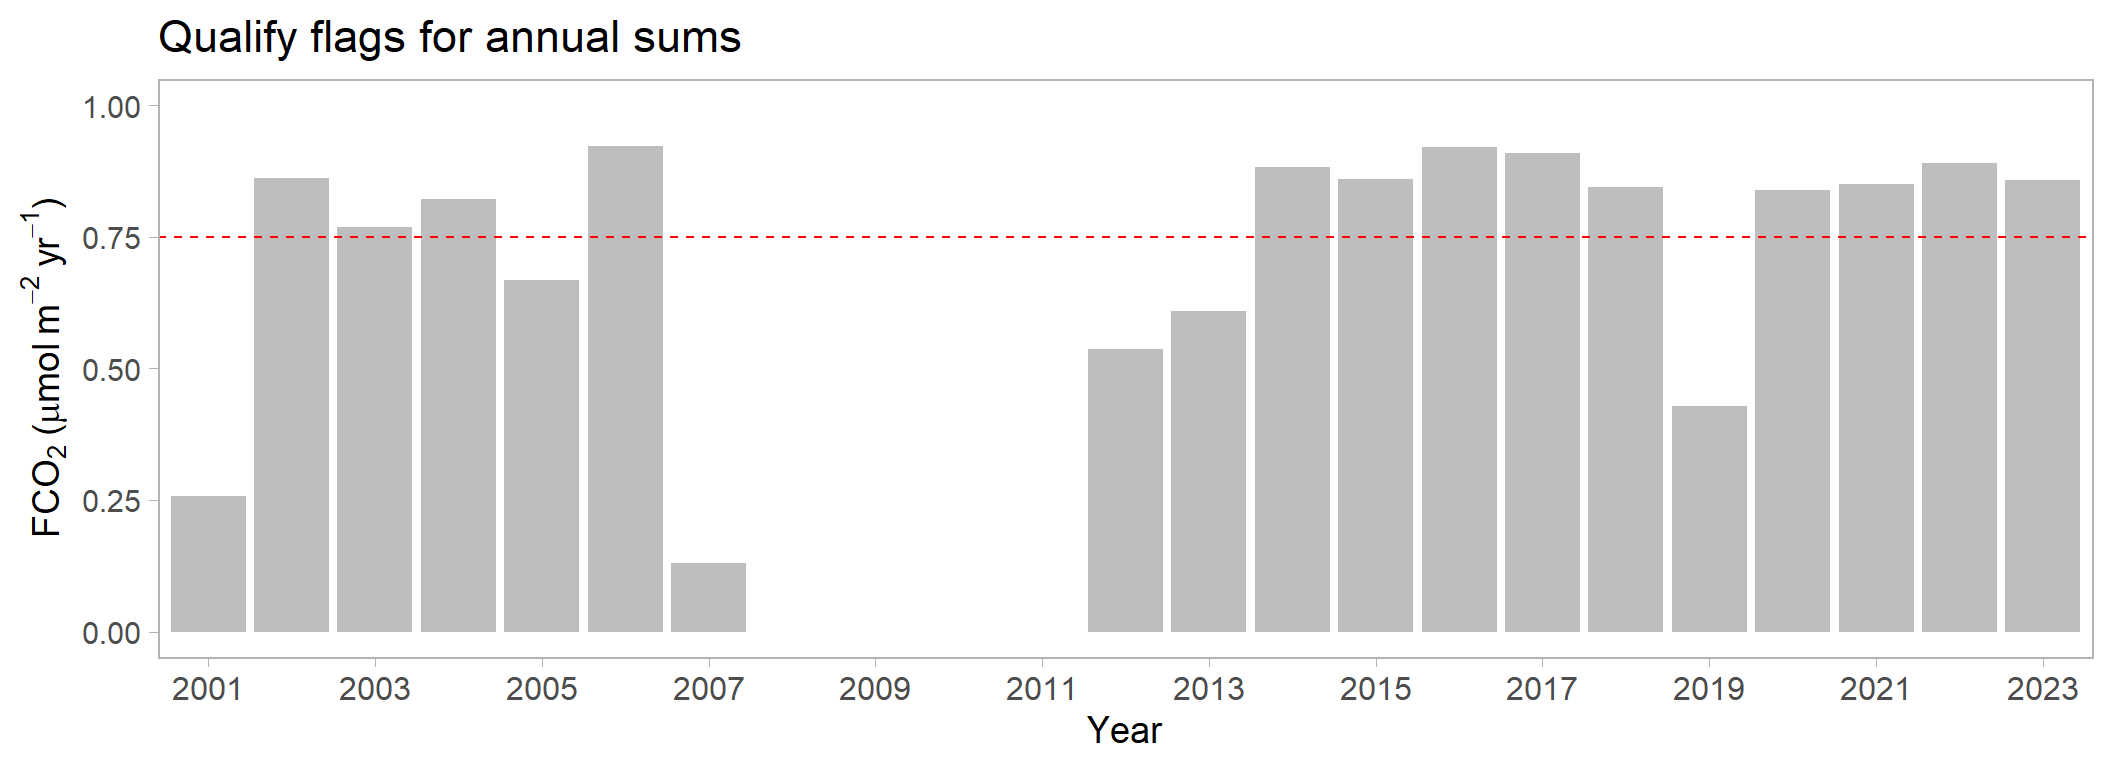
\includegraphics{FLUXNET_files/figure-latex/unnamed-chunk-4-2.pdf}

\subsection{Computing monthly sums}\label{computing-monthly-sums}

\begin{Shaded}
\begin{Highlighting}[]
\NormalTok{lambda }\OtherTok{\textless{}{-}} \FloatTok{2.45e6}  \CommentTok{\# Latent heat of vaporization (J/kg)}
\NormalTok{sec\_per\_30min }\OtherTok{\textless{}{-}} \DecValTok{30}\SpecialCharTok{*}\DecValTok{60}  \CommentTok{\# Seconds in 30 minutes}

\CommentTok{\# Conversion factor for converting µmol CO2 m{-}2 s{-}1 to gC per 30 min}
\NormalTok{conversion\_factor\_C }\OtherTok{\textless{}{-}}\NormalTok{ (}\DecValTok{12} \SpecialCharTok{*} \DecValTok{10}\SpecialCharTok{\^{}}\NormalTok{(}\SpecialCharTok{{-}}\DecValTok{3}\NormalTok{)) }\SpecialCharTok{*} \DecValTok{1800} \SpecialCharTok{/} \DecValTok{1000}  \CommentTok{\# (mg C per µmol) * (sec per 30 min) / (mg to g)}


\NormalTok{df.HH }\OtherTok{\textless{}{-}}\NormalTok{ df.HH }\SpecialCharTok{\%\textgreater{}\%}
  \FunctionTok{mutate}\NormalTok{(}\AttributeTok{ET =}\NormalTok{ (LE\_F\_MDS }\SpecialCharTok{/}\NormalTok{ lambda) }\SpecialCharTok{*}\NormalTok{ sec\_per\_30min) }\CommentTok{\# convert unit from  W m{-}2 to mm}
\CommentTok{\# Summarize the data by year and month for NEE, GPP, RECO, and additional variables}
\DocumentationTok{\#\# For NEE, GPP, and Reco, converting unit from µmolCO2 mol{-}1 to g C m{-}2 month{-}1}
\NormalTok{monthly\_data }\OtherTok{\textless{}{-}}\NormalTok{ df.HH }\SpecialCharTok{\%\textgreater{}\%}
  \FunctionTok{group\_by}\NormalTok{(year, month) }\SpecialCharTok{\%\textgreater{}\%}
  \FunctionTok{summarise}\NormalTok{(}
    \AttributeTok{NEE =} \FunctionTok{sum}\NormalTok{(NEE\_VUT\_REF }\SpecialCharTok{*}\NormalTok{ conversion\_factor\_C, }\AttributeTok{na.rm =} \ConstantTok{TRUE}\NormalTok{), }
    \AttributeTok{GPP =} \SpecialCharTok{{-}}\FunctionTok{sum}\NormalTok{(GPP\_DT\_VUT\_REF }\SpecialCharTok{*}\NormalTok{ conversion\_factor\_C, }\AttributeTok{na.rm =} \ConstantTok{TRUE}\NormalTok{),}
    \AttributeTok{RECO =} \FunctionTok{sum}\NormalTok{(RECO\_DT\_VUT\_REF }\SpecialCharTok{*}\NormalTok{ conversion\_factor\_C, }\AttributeTok{na.rm =} \ConstantTok{TRUE}\NormalTok{),}
    \AttributeTok{P =} \FunctionTok{sum}\NormalTok{(P\_F, }\AttributeTok{na.rm =} \ConstantTok{TRUE}\NormalTok{),}
    \AttributeTok{ET =} \FunctionTok{sum}\NormalTok{(ET, }\AttributeTok{na.rm =} \ConstantTok{TRUE}\NormalTok{),}
    \AttributeTok{NETRAD =} \FunctionTok{sum}\NormalTok{(NETRAD, }\AttributeTok{na.rm =} \ConstantTok{TRUE}\NormalTok{) }\SpecialCharTok{/}\NormalTok{ (}\FunctionTok{n}\NormalTok{() }\SpecialCharTok{*} \FloatTok{0.5}\NormalTok{),  }\CommentTok{\# Convert to W/m²}
    \AttributeTok{LE =} \FunctionTok{sum}\NormalTok{(LE\_F\_MDS, }\AttributeTok{na.rm =} \ConstantTok{TRUE}\NormalTok{) }\SpecialCharTok{/}\NormalTok{ (}\FunctionTok{n}\NormalTok{() }\SpecialCharTok{*} \FloatTok{0.5}\NormalTok{),  }\CommentTok{\# Convert to W/m²}
    \AttributeTok{H =} \FunctionTok{sum}\NormalTok{(H\_F\_MDS, }\AttributeTok{na.rm =} \ConstantTok{TRUE}\NormalTok{) }\SpecialCharTok{/}\NormalTok{ (}\FunctionTok{n}\NormalTok{() }\SpecialCharTok{*} \FloatTok{0.5}\NormalTok{),  }\CommentTok{\# Convert to W/m²}
    \AttributeTok{SW\_IN =} \FunctionTok{sum}\NormalTok{(SW\_IN\_F, }\AttributeTok{na.rm =} \ConstantTok{TRUE}\NormalTok{) }\SpecialCharTok{/}\NormalTok{ (}\FunctionTok{n}\NormalTok{() }\SpecialCharTok{*} \FloatTok{0.5}\NormalTok{),  }\CommentTok{\# Convert to W/m²}
    \AttributeTok{Tair =} \FunctionTok{median}\NormalTok{(TA\_F, }\AttributeTok{na.rm =} \ConstantTok{TRUE}\NormalTok{),  }\CommentTok{\# Monthly average of air temperature}
    \AttributeTok{.groups =} \StringTok{"drop"}
\NormalTok{  ) }\SpecialCharTok{\%\textgreater{}\%}
  \FunctionTok{mutate}\NormalTok{(}
    \AttributeTok{month\_year =} \FunctionTok{as.Date}\NormalTok{(}\FunctionTok{paste}\NormalTok{(year, month, }\DecValTok{1}\NormalTok{, }\AttributeTok{sep =} \StringTok{"{-}"}\NormalTok{)),}
    \AttributeTok{year\_label\_pos =} \FunctionTok{as.Date}\NormalTok{(}\FunctionTok{paste}\NormalTok{(year, }\StringTok{"07"}\NormalTok{, }\StringTok{"01"}\NormalTok{, }\AttributeTok{sep =} \StringTok{"{-}"}\NormalTok{)),}
    \AttributeTok{y\_label\_pos =} \FunctionTok{max}\NormalTok{(GPP, RECO, NEE, }\AttributeTok{na.rm =} \ConstantTok{TRUE}\NormalTok{) }\SpecialCharTok{*} \FloatTok{1.2}
\NormalTok{  ) }
\end{Highlighting}
\end{Shaded}

\subsection{Figure 3: monthly meterological
variables}\label{figure-3-monthly-meterological-variables}

\begin{Shaded}
\begin{Highlighting}[]
\CommentTok{\# Tair {-}{-}{-}{-}{-}{-}{-}{-}{-}{-}{-}{-}{-}{-}{-}{-}{-}{-}{-}{-}{-}{-}{-}{-}{-}{-}{-}{-}{-}{-}{-}{-}{-}{-}{-}{-}{-}{-}{-}{-}{-}{-}{-}{-}{-}{-}{-}{-}{-}{-}{-}{-}{-}}
\NormalTok{monthly\_data }\OtherTok{\textless{}{-}}\NormalTok{ monthly\_data }\SpecialCharTok{\%\textgreater{}\%}
  \FunctionTok{mutate}\NormalTok{(}\AttributeTok{y\_label\_pos =} \FunctionTok{max}\NormalTok{(Tair, }\AttributeTok{na.rm =} \ConstantTok{TRUE}\NormalTok{) }\SpecialCharTok{*} \FloatTok{1.2}\NormalTok{)}

\FunctionTok{ggplot}\NormalTok{(monthly\_data, }\FunctionTok{aes}\NormalTok{(}\AttributeTok{x =}\NormalTok{ month\_year)) }\SpecialCharTok{+}
  \CommentTok{\# Add continuous lines and dots for Tair}
  \FunctionTok{geom\_line}\NormalTok{(}\FunctionTok{aes}\NormalTok{(}\AttributeTok{y =}\NormalTok{ Tair, }\AttributeTok{color =} \StringTok{"Tair"}\NormalTok{), }\AttributeTok{size =} \DecValTok{1}\NormalTok{) }\SpecialCharTok{+}
  \FunctionTok{geom\_point}\NormalTok{(}\FunctionTok{aes}\NormalTok{(}\AttributeTok{y =}\NormalTok{ Tair, }\AttributeTok{color =} \StringTok{"Tair"}\NormalTok{), }\AttributeTok{size =} \DecValTok{3}\NormalTok{) }\SpecialCharTok{+}
  
  \CommentTok{\# Add horizontal dashed line at 0°C}
  \FunctionTok{geom\_hline}\NormalTok{(}\AttributeTok{yintercept =} \DecValTok{0}\NormalTok{, }\AttributeTok{linetype =} \StringTok{"dashed"}\NormalTok{, }\AttributeTok{color =} \StringTok{"black"}\NormalTok{, }\AttributeTok{size =} \FloatTok{0.8}\NormalTok{) }\SpecialCharTok{+}
  
  \CommentTok{\# Add vertical dashed lines at the end of each year}
  \FunctionTok{geom\_vline}\NormalTok{(}\AttributeTok{data =}\NormalTok{ monthly\_data }\SpecialCharTok{\%\textgreater{}\%} \FunctionTok{filter}\NormalTok{(month }\SpecialCharTok{==} \DecValTok{12}\NormalTok{), }
             \FunctionTok{aes}\NormalTok{(}\AttributeTok{xintercept =} \FunctionTok{as.numeric}\NormalTok{(month\_year) }\SpecialCharTok{+} \DecValTok{15}\NormalTok{), }
             \AttributeTok{linetype =} \StringTok{"dashed"}\NormalTok{, }\AttributeTok{color =} \StringTok{"gray"}\NormalTok{, }\AttributeTok{size =} \FloatTok{0.5}\NormalTok{) }\SpecialCharTok{+}
  
  \CommentTok{\# Fix year labels position}
  \FunctionTok{geom\_text}\NormalTok{(}\AttributeTok{data =}\NormalTok{ monthly\_data }\SpecialCharTok{\%\textgreater{}\%} \FunctionTok{filter}\NormalTok{(month }\SpecialCharTok{==} \DecValTok{6}\NormalTok{), }
            \FunctionTok{aes}\NormalTok{(}\AttributeTok{x =}\NormalTok{ year\_label\_pos, }\AttributeTok{label =}\NormalTok{ year), }
            \AttributeTok{y =} \FunctionTok{max}\NormalTok{(monthly\_data}\SpecialCharTok{$}\NormalTok{Tair, }\AttributeTok{na.rm =} \ConstantTok{TRUE}\NormalTok{) }\SpecialCharTok{*} \FloatTok{1.2}\NormalTok{, }
            \AttributeTok{color =} \StringTok{"black"}\NormalTok{, }\AttributeTok{size =} \DecValTok{5}\NormalTok{, }\AttributeTok{fontface =} \StringTok{"bold"}\NormalTok{) }\SpecialCharTok{+}
  
  \CommentTok{\# Customize the plot}
  \FunctionTok{labs}\NormalTok{(}\AttributeTok{x =} \StringTok{"Month"}\NormalTok{, }\AttributeTok{y =} \FunctionTok{expression}\NormalTok{(}\StringTok{"Air Temperature (°C)"}\NormalTok{), }\AttributeTok{title =} \StringTok{"Monthly Air Temperature Trend"}\NormalTok{) }\SpecialCharTok{+}
  \FunctionTok{scale\_color\_manual}\NormalTok{(}\AttributeTok{values =} \FunctionTok{c}\NormalTok{(}\StringTok{"Tair"} \OtherTok{=} \StringTok{"orange"}\NormalTok{)) }\SpecialCharTok{+}
  \FunctionTok{scale\_x\_date}\NormalTok{(}\AttributeTok{date\_labels =} \StringTok{"\%m"}\NormalTok{, }\AttributeTok{date\_breaks =} \StringTok{"6 month"}\NormalTok{, }\AttributeTok{expand =} \FunctionTok{c}\NormalTok{(}\DecValTok{0}\NormalTok{, }\DecValTok{0}\NormalTok{)) }\SpecialCharTok{+}  \CommentTok{\# Continuous months}
  \FunctionTok{scale\_y\_continuous}\NormalTok{(}
    \AttributeTok{breaks =} \FunctionTok{seq}\NormalTok{(}\FunctionTok{floor}\NormalTok{(}\FunctionTok{min}\NormalTok{(monthly\_data}\SpecialCharTok{$}\NormalTok{Tair, }\AttributeTok{na.rm =} \ConstantTok{TRUE}\NormalTok{) }\SpecialCharTok{/} \DecValTok{10}\NormalTok{) }\SpecialCharTok{*} \DecValTok{10}\NormalTok{, }
                 \FunctionTok{ceiling}\NormalTok{(}\FunctionTok{max}\NormalTok{(monthly\_data}\SpecialCharTok{$}\NormalTok{Tair, }\AttributeTok{na.rm =} \ConstantTok{TRUE}\NormalTok{) }\SpecialCharTok{/} \DecValTok{10}\NormalTok{) }\SpecialCharTok{*} \DecValTok{10}\NormalTok{, }
                 \AttributeTok{by =} \DecValTok{4}\NormalTok{),}
    \AttributeTok{limits =} \FunctionTok{c}\NormalTok{(}\FunctionTok{floor}\NormalTok{(}\FunctionTok{min}\NormalTok{(monthly\_data}\SpecialCharTok{$}\NormalTok{Tair, }\AttributeTok{na.rm =} \ConstantTok{TRUE}\NormalTok{)) }\SpecialCharTok{{-}} \DecValTok{5}\NormalTok{, }
               \FunctionTok{ceiling}\NormalTok{(}\FunctionTok{max}\NormalTok{(monthly\_data}\SpecialCharTok{$}\NormalTok{Tair, }\AttributeTok{na.rm =} \ConstantTok{TRUE}\NormalTok{)) }\SpecialCharTok{+} \DecValTok{5}\NormalTok{)}
\NormalTok{  ) }\SpecialCharTok{+}\NormalTok{ my\_theme}
\end{Highlighting}
\end{Shaded}

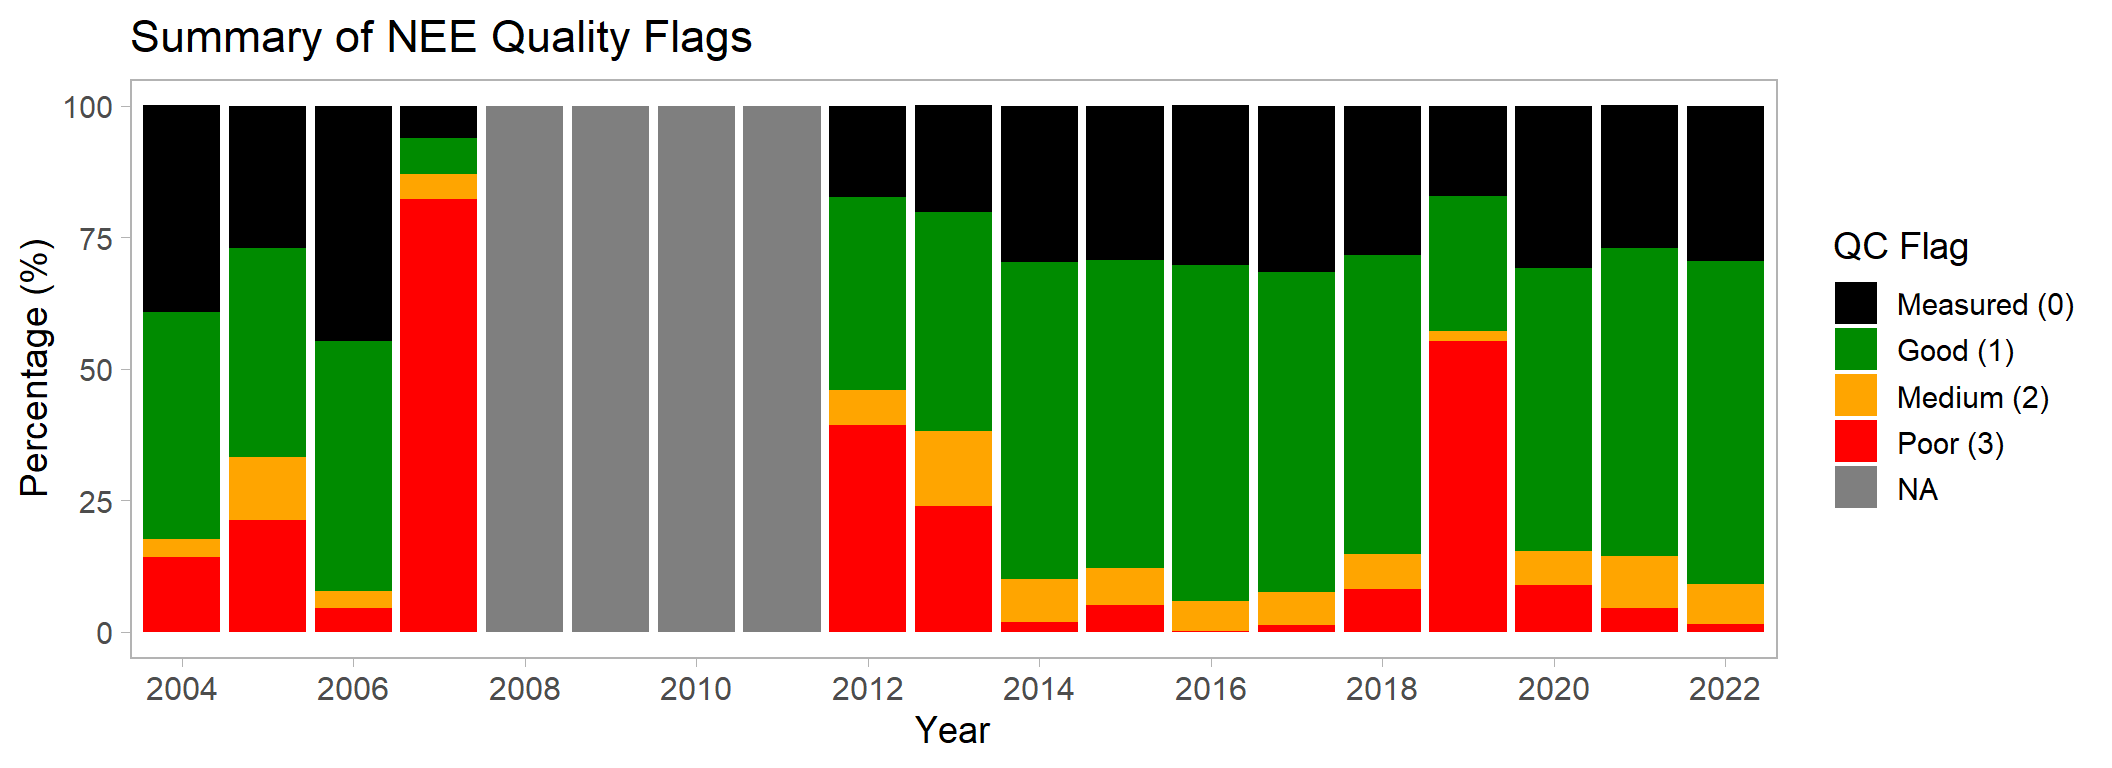
\includegraphics{FLUXNET_files/figure-latex/unnamed-chunk-6-1.pdf}

\begin{Shaded}
\begin{Highlighting}[]
\CommentTok{\# Incoming shortwave radiation {-}{-}{-}{-}{-}{-}{-}{-}{-}{-}{-}{-}{-}{-}{-}{-}{-}{-}{-}{-}{-}{-}{-}{-}{-}{-}{-}{-}{-}{-}{-}{-}{-}{-}{-}{-}{-}{-}{-}{-}{-}{-}{-}{-}{-}{-}{-}{-}{-}{-}{-}{-}{-}}
\NormalTok{monthly\_data }\OtherTok{\textless{}{-}}\NormalTok{ monthly\_data }\SpecialCharTok{\%\textgreater{}\%}
  \FunctionTok{mutate}\NormalTok{(}\AttributeTok{y\_label\_pos =} \FunctionTok{max}\NormalTok{(SW\_IN, }\AttributeTok{na.rm =} \ConstantTok{TRUE}\NormalTok{) }\SpecialCharTok{*} \DecValTok{1}\NormalTok{)}

\FunctionTok{ggplot}\NormalTok{(monthly\_data, }\FunctionTok{aes}\NormalTok{(}\AttributeTok{x =}\NormalTok{ month\_year)) }\SpecialCharTok{+}
  \CommentTok{\# Add continuous lines and dots for SW\_IN}
  \FunctionTok{geom\_line}\NormalTok{(}\FunctionTok{aes}\NormalTok{(}\AttributeTok{y =}\NormalTok{ SW\_IN, }\AttributeTok{color =} \StringTok{"SW\_IN"}\NormalTok{), }\AttributeTok{size =} \DecValTok{1}\NormalTok{) }\SpecialCharTok{+}
  \FunctionTok{geom\_point}\NormalTok{(}\FunctionTok{aes}\NormalTok{(}\AttributeTok{y =}\NormalTok{ SW\_IN, }\AttributeTok{color =} \StringTok{"SW\_IN"}\NormalTok{), }\AttributeTok{size =} \DecValTok{3}\NormalTok{) }\SpecialCharTok{+}
  
  \CommentTok{\# Add horizontal dashed line at 0}
  \FunctionTok{geom\_hline}\NormalTok{(}\AttributeTok{yintercept =} \DecValTok{0}\NormalTok{, }\AttributeTok{linetype =} \StringTok{"dashed"}\NormalTok{, }\AttributeTok{color =} \StringTok{"black"}\NormalTok{, }\AttributeTok{size =} \FloatTok{0.8}\NormalTok{) }\SpecialCharTok{+}
  
  \CommentTok{\# Add vertical dashed lines at the end of each year}
  \FunctionTok{geom\_vline}\NormalTok{(}\AttributeTok{data =}\NormalTok{ monthly\_data }\SpecialCharTok{\%\textgreater{}\%} \FunctionTok{filter}\NormalTok{(month }\SpecialCharTok{==} \DecValTok{12}\NormalTok{), }
             \FunctionTok{aes}\NormalTok{(}\AttributeTok{xintercept =} \FunctionTok{as.numeric}\NormalTok{(month\_year) }\SpecialCharTok{+} \DecValTok{15}\NormalTok{), }
             \AttributeTok{linetype =} \StringTok{"dashed"}\NormalTok{, }\AttributeTok{color =} \StringTok{"gray"}\NormalTok{, }\AttributeTok{size =} \FloatTok{0.5}\NormalTok{) }\SpecialCharTok{+}
  
  \CommentTok{\# Fix year labels position}
  \FunctionTok{geom\_text}\NormalTok{(}\AttributeTok{data =}\NormalTok{ monthly\_data }\SpecialCharTok{\%\textgreater{}\%} \FunctionTok{filter}\NormalTok{(month }\SpecialCharTok{==} \DecValTok{6}\NormalTok{), }
            \FunctionTok{aes}\NormalTok{(}\AttributeTok{x =}\NormalTok{ year\_label\_pos, }\AttributeTok{label =}\NormalTok{ year), }
            \AttributeTok{y =} \FunctionTok{max}\NormalTok{(monthly\_data}\SpecialCharTok{$}\NormalTok{SW\_IN, }\AttributeTok{na.rm =} \ConstantTok{TRUE}\NormalTok{) }\SpecialCharTok{*} \DecValTok{1}\NormalTok{, }
            \AttributeTok{color =} \StringTok{"black"}\NormalTok{, }\AttributeTok{size =} \DecValTok{5}\NormalTok{, }\AttributeTok{fontface =} \StringTok{"bold"}\NormalTok{) }\SpecialCharTok{+}
  
  \CommentTok{\# Customize the plot}
  \FunctionTok{labs}\NormalTok{(}\AttributeTok{x =} \StringTok{"Month"}\NormalTok{, }\AttributeTok{y =} \FunctionTok{expression}\NormalTok{(}\StringTok{"Incoming Shortwave Radiation (W/m²)"}\NormalTok{), }
       \AttributeTok{title =} \StringTok{"Monthly Incoming Shortwave Trend"}\NormalTok{) }\SpecialCharTok{+}
  \FunctionTok{scale\_color\_manual}\NormalTok{(}\AttributeTok{values =} \FunctionTok{c}\NormalTok{(}\StringTok{"SW\_IN"} \OtherTok{=} \StringTok{"blue"}\NormalTok{)) }\SpecialCharTok{+}
  \FunctionTok{scale\_x\_date}\NormalTok{(}\AttributeTok{date\_labels =} \StringTok{"\%m"}\NormalTok{, }\AttributeTok{date\_breaks =} \StringTok{"6 month"}\NormalTok{, }\AttributeTok{expand =} \FunctionTok{c}\NormalTok{(}\DecValTok{0}\NormalTok{, }\DecValTok{0}\NormalTok{)) }\SpecialCharTok{+}  
  \FunctionTok{scale\_y\_continuous}\NormalTok{(}
    \AttributeTok{breaks =} \FunctionTok{seq}\NormalTok{(}\DecValTok{0}\NormalTok{, }
                 \FunctionTok{ceiling}\NormalTok{(}\FunctionTok{max}\NormalTok{(monthly\_data}\SpecialCharTok{$}\NormalTok{SW\_IN, }\AttributeTok{na.rm =} \ConstantTok{TRUE}\NormalTok{) }\SpecialCharTok{/} \DecValTok{10}\NormalTok{) }\SpecialCharTok{*} \DecValTok{10}\NormalTok{, }
                 \AttributeTok{by =} \DecValTok{50}\NormalTok{),}
    \AttributeTok{limits =} \FunctionTok{c}\NormalTok{(}\DecValTok{0}\NormalTok{, }\FunctionTok{ceiling}\NormalTok{(}\FunctionTok{max}\NormalTok{(monthly\_data}\SpecialCharTok{$}\NormalTok{SW\_IN, }\AttributeTok{na.rm =} \ConstantTok{TRUE}\NormalTok{)) }\SpecialCharTok{+} \DecValTok{5}\NormalTok{)}
\NormalTok{  ) }\SpecialCharTok{+}\NormalTok{ my\_theme}
\end{Highlighting}
\end{Shaded}

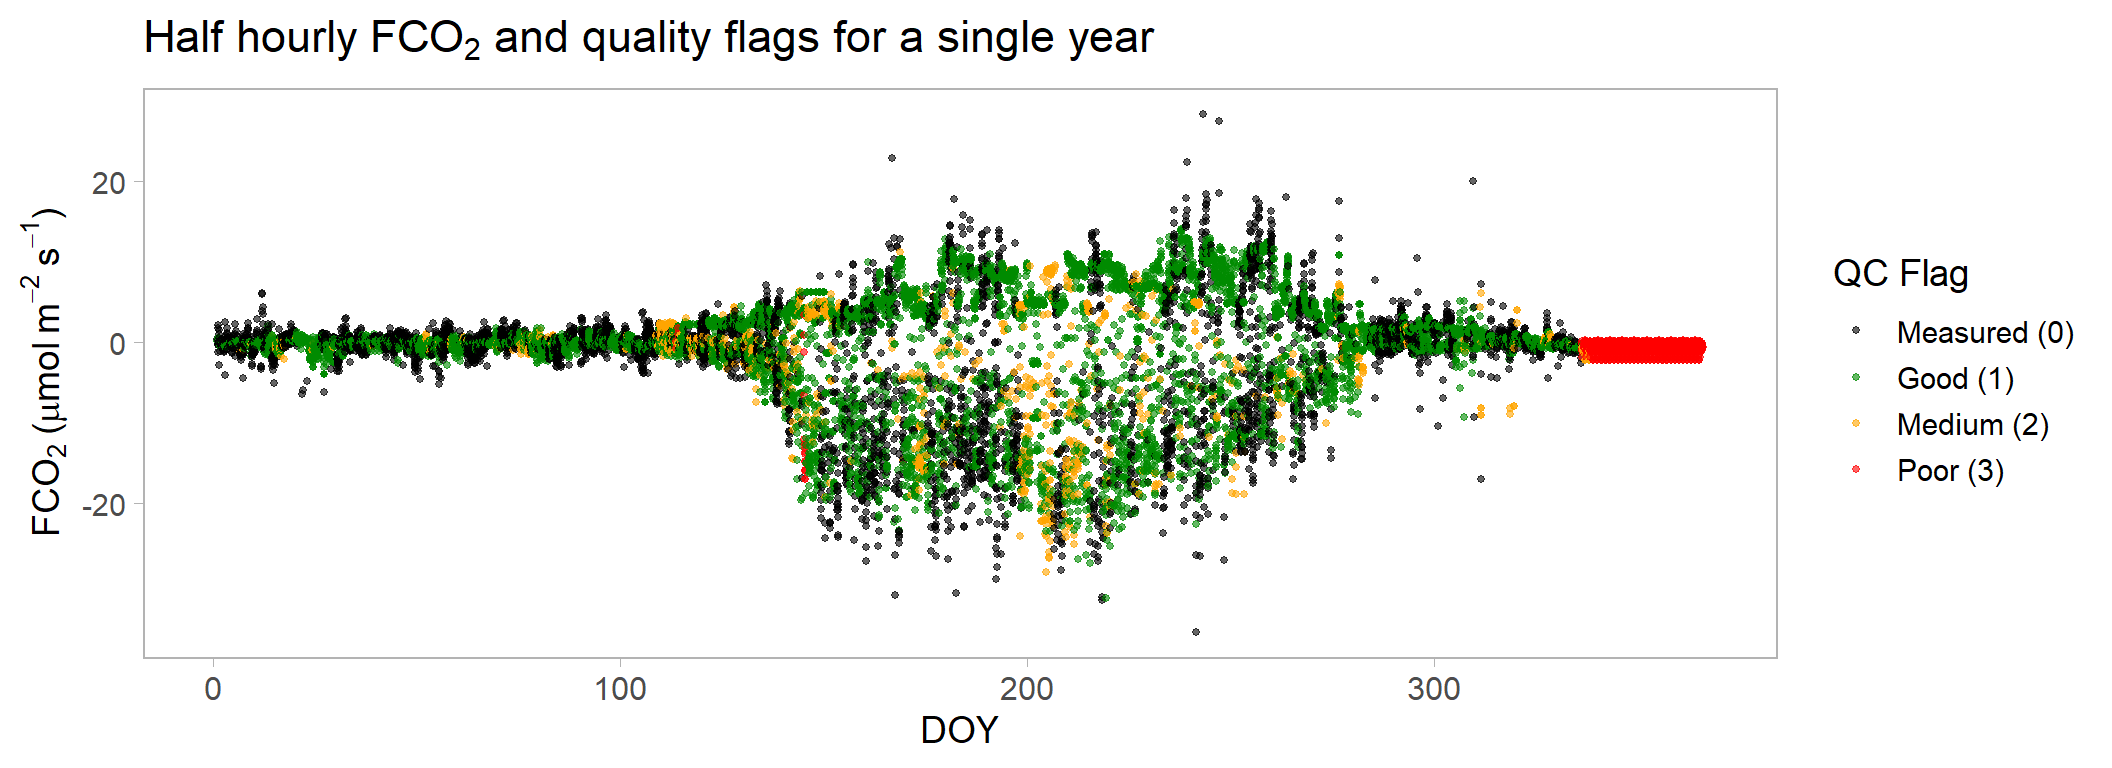
\includegraphics{FLUXNET_files/figure-latex/unnamed-chunk-6-2.pdf}

\subsection{Figure 4: Monthly NEE, GPP, RECO (to be updated with Mo's
figure)}\label{figure-4-monthly-nee-gpp-reco-to-be-updated-with-mos-figure}

\begin{Shaded}
\begin{Highlighting}[]
\NormalTok{monthly\_data }\OtherTok{\textless{}{-}}\NormalTok{ monthly\_data }\SpecialCharTok{\%\textgreater{}\%}
  \FunctionTok{mutate}\NormalTok{(}\AttributeTok{y\_label\_pos =} \FunctionTok{max}\NormalTok{(GPP,RECO, NEE, }\AttributeTok{na.rm =} \ConstantTok{TRUE}\NormalTok{) }\SpecialCharTok{*} \DecValTok{1}\NormalTok{)}

\FunctionTok{ggplot}\NormalTok{(monthly\_data, }\FunctionTok{aes}\NormalTok{(}\AttributeTok{x =}\NormalTok{ month\_year)) }\SpecialCharTok{+}
  \CommentTok{\# Add bars for GPP and RECO}
  \FunctionTok{geom\_bar}\NormalTok{(}\FunctionTok{aes}\NormalTok{(}\AttributeTok{y =}\NormalTok{ GPP, }\AttributeTok{fill =} \StringTok{"GPP"}\NormalTok{), }\AttributeTok{stat =} \StringTok{"identity"}\NormalTok{, }\AttributeTok{position =} \StringTok{"dodge"}\NormalTok{) }\SpecialCharTok{+}
  \FunctionTok{geom\_bar}\NormalTok{(}\FunctionTok{aes}\NormalTok{(}\AttributeTok{y =}\NormalTok{ RECO, }\AttributeTok{fill =} \StringTok{"RECO"}\NormalTok{), }\AttributeTok{stat =} \StringTok{"identity"}\NormalTok{, }\AttributeTok{position =} \StringTok{"dodge"}\NormalTok{) }\SpecialCharTok{+}
  
  \CommentTok{\# Add continuous line and dots for NEE}
  \FunctionTok{geom\_line}\NormalTok{(}\FunctionTok{aes}\NormalTok{(}\AttributeTok{y =}\NormalTok{ NEE, }\AttributeTok{color =} \StringTok{"NEE"}\NormalTok{), }\AttributeTok{size =} \DecValTok{1}\NormalTok{) }\SpecialCharTok{+}
  \FunctionTok{geom\_point}\NormalTok{(}\FunctionTok{aes}\NormalTok{(}\AttributeTok{y =}\NormalTok{ NEE, }\AttributeTok{color =} \StringTok{"NEE"}\NormalTok{), }\AttributeTok{size =} \DecValTok{3}\NormalTok{) }\SpecialCharTok{+}
  
  \CommentTok{\# Add vertical dashed lines at the end of each year}
  \FunctionTok{geom\_vline}\NormalTok{(}\AttributeTok{data =}\NormalTok{ monthly\_data }\SpecialCharTok{\%\textgreater{}\%} \FunctionTok{filter}\NormalTok{(month }\SpecialCharTok{==} \DecValTok{12}\NormalTok{), }
             \FunctionTok{aes}\NormalTok{(}\AttributeTok{xintercept =} \FunctionTok{as.numeric}\NormalTok{(month\_year) }\SpecialCharTok{+} \DecValTok{15}\NormalTok{), }
             \AttributeTok{linetype =} \StringTok{"dashed"}\NormalTok{, }\AttributeTok{color =} \StringTok{"black"}\NormalTok{, }\AttributeTok{size =} \FloatTok{0.5}\NormalTok{) }\SpecialCharTok{+}

  \CommentTok{\# Move year labels higher}
  \FunctionTok{geom\_text}\NormalTok{(}\AttributeTok{data =}\NormalTok{ monthly\_data }\SpecialCharTok{\%\textgreater{}\%} \FunctionTok{filter}\NormalTok{(month }\SpecialCharTok{==} \DecValTok{6}\NormalTok{), }
            \FunctionTok{aes}\NormalTok{(}\AttributeTok{x =}\NormalTok{ year\_label\_pos, }\AttributeTok{y =}\NormalTok{ y\_label\_pos, }\AttributeTok{label =}\NormalTok{ year), }
            \AttributeTok{color =} \StringTok{"black"}\NormalTok{, }\AttributeTok{size =} \DecValTok{5}\NormalTok{, }\AttributeTok{fontface =} \StringTok{"bold"}\NormalTok{) }\SpecialCharTok{+}
  
  \CommentTok{\# Define colors for bars and lines}
  \FunctionTok{scale\_fill\_manual}\NormalTok{(}\AttributeTok{values =} \FunctionTok{c}\NormalTok{(}\StringTok{"GPP"} \OtherTok{=} \StringTok{"\#00BFC4"}\NormalTok{, }\StringTok{"RECO"} \OtherTok{=} \StringTok{"\#F8766D"}\NormalTok{)) }\SpecialCharTok{+}
  \FunctionTok{scale\_color\_manual}\NormalTok{(}\AttributeTok{values =} \FunctionTok{c}\NormalTok{(}\StringTok{"NEE"} \OtherTok{=} \StringTok{"purple"}\NormalTok{)) }\SpecialCharTok{+}
  
  \CommentTok{\# Scale for the left y{-}axis (Carbon fluxes)}
  \FunctionTok{scale\_y\_continuous}\NormalTok{(}
    \AttributeTok{name =} \FunctionTok{expression}\NormalTok{(}\StringTok{"g C per month"}\SpecialCharTok{\^{}}\DecValTok{2}\NormalTok{),}
    \AttributeTok{breaks =} \FunctionTok{seq}\NormalTok{(}\FunctionTok{floor}\NormalTok{(}\FunctionTok{min}\NormalTok{(monthly\_data}\SpecialCharTok{$}\NormalTok{NEE, monthly\_data}\SpecialCharTok{$}\NormalTok{GPP, monthly\_data}\SpecialCharTok{$}\NormalTok{RECO, }\AttributeTok{na.rm =} \ConstantTok{TRUE}\NormalTok{) }\SpecialCharTok{/} \DecValTok{50}\NormalTok{) }\SpecialCharTok{*} \DecValTok{50}\NormalTok{, }
                 \FunctionTok{ceiling}\NormalTok{(}\FunctionTok{max}\NormalTok{(monthly\_data}\SpecialCharTok{$}\NormalTok{NEE, monthly\_data}\SpecialCharTok{$}\NormalTok{GPP, monthly\_data}\SpecialCharTok{$}\NormalTok{RECO, }\AttributeTok{na.rm =} \ConstantTok{TRUE}\NormalTok{) }\SpecialCharTok{/} \DecValTok{50}\NormalTok{) }\SpecialCharTok{*} \DecValTok{50}\NormalTok{, }
                 \AttributeTok{by =} \DecValTok{20}\NormalTok{),}
\NormalTok{    )}\SpecialCharTok{+}
  \CommentTok{\# X{-}axis settings}
  \FunctionTok{scale\_x\_date}\NormalTok{(}\AttributeTok{date\_labels =} \StringTok{"\%m"}\NormalTok{, }\AttributeTok{date\_breaks =} \StringTok{"6 month"}\NormalTok{, }\AttributeTok{expand =} \FunctionTok{c}\NormalTok{(}\DecValTok{0}\NormalTok{, }\DecValTok{0}\NormalTok{)) }\SpecialCharTok{+}\NormalTok{  my\_theme}
\end{Highlighting}
\end{Shaded}

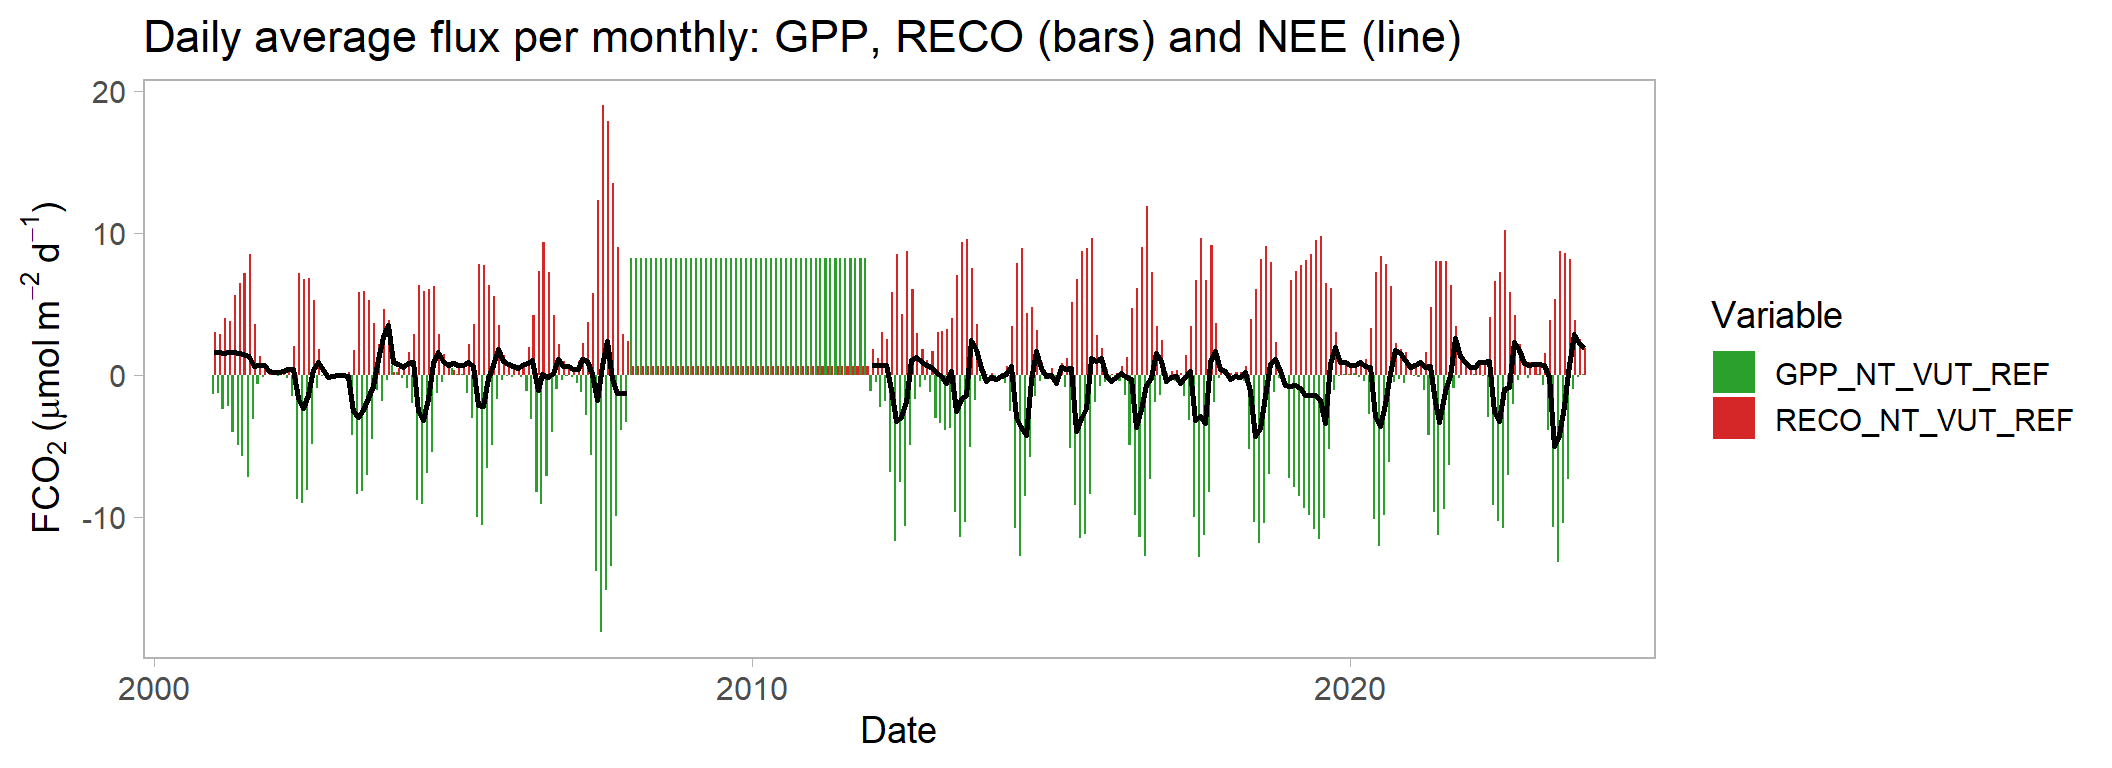
\includegraphics{FLUXNET_files/figure-latex/unnamed-chunk-7-1.pdf} Where
to go from here: - Interpret the figures and include them in your group
presentation. You can also create your own figures: - plot monthly
anomalies of meteorological variables. - plot diural patterns of
meteorological variables.

\section{Inspect Qualify flags}\label{inspect-qualify-flags}

\begin{Shaded}
\begin{Highlighting}[]
\NormalTok{df.HH }\OtherTok{\textless{}{-}}\NormalTok{ df.HH }\SpecialCharTok{\%\textgreater{}\%} \CommentTok{\# using half{-}hourly data}
  \FunctionTok{mutate}\NormalTok{(}
    \AttributeTok{year =} \FunctionTok{year}\NormalTok{(TIMESTAMP\_END),}
    \AttributeTok{DOY =} \FunctionTok{yday}\NormalTok{(TIMESTAMP\_END) }\SpecialCharTok{+} 
\NormalTok{      (}\FunctionTok{hour}\NormalTok{(TIMESTAMP\_END) }\SpecialCharTok{+} \FunctionTok{minute}\NormalTok{(TIMESTAMP\_END)}\SpecialCharTok{/}\DecValTok{60} \SpecialCharTok{+} \FunctionTok{second}\NormalTok{(TIMESTAMP\_END)}\SpecialCharTok{/}\DecValTok{3600}\NormalTok{) }\SpecialCharTok{/} \DecValTok{24}\NormalTok{,}
    \AttributeTok{qc\_label =} \FunctionTok{factor}\NormalTok{(}
\NormalTok{      NEE\_VUT\_REF\_QC,}
      \AttributeTok{levels =} \FunctionTok{c}\NormalTok{(}\DecValTok{0}\NormalTok{, }\DecValTok{1}\NormalTok{, }\DecValTok{2}\NormalTok{, }\DecValTok{3}\NormalTok{),}
      \AttributeTok{labels =} \FunctionTok{c}\NormalTok{(}\StringTok{"Measured (0)"}\NormalTok{, }\StringTok{"Good (1)"}\NormalTok{, }\StringTok{"Medium (2)"}\NormalTok{, }\StringTok{"Poor (3)"}\NormalTok{)}
\NormalTok{    )}
\NormalTok{  )}

\CommentTok{\#calculate the percentage of each flag}
\NormalTok{qc\_summary }\OtherTok{\textless{}{-}}\NormalTok{ df.HH }\SpecialCharTok{\%\textgreater{}\%}
  \FunctionTok{group\_by}\NormalTok{(year, qc\_label) }\SpecialCharTok{\%\textgreater{}\%}
  \FunctionTok{summarise}\NormalTok{(}\AttributeTok{count =} \FunctionTok{n}\NormalTok{(), }\AttributeTok{.groups =} \StringTok{"drop"}\NormalTok{) }\SpecialCharTok{\%\textgreater{}\%}
  \FunctionTok{group\_by}\NormalTok{(year) }\SpecialCharTok{\%\textgreater{}\%}
  \FunctionTok{mutate}\NormalTok{(}
    \AttributeTok{total =} \FunctionTok{sum}\NormalTok{(count),}
    \AttributeTok{percent =} \FunctionTok{round}\NormalTok{(}\DecValTok{100} \SpecialCharTok{*}\NormalTok{ count }\SpecialCharTok{/}\NormalTok{ total, }\DecValTok{1}\NormalTok{),}
    \AttributeTok{label =} \FunctionTok{paste0}\NormalTok{(qc\_label, }\StringTok{": "}\NormalTok{, percent, }\StringTok{"\%"}\NormalTok{)}
\NormalTok{  )}
\CommentTok{\# View(qc\_summary)}

\CommentTok{\# plot qc\_summary by year}
\NormalTok{qc\_summary }\SpecialCharTok{\%\textgreater{}\%}
  \FunctionTok{filter}\NormalTok{(year }\SpecialCharTok{\textgreater{}=} \DecValTok{2004}\NormalTok{, year }\SpecialCharTok{\textless{}=} \DecValTok{2022}\NormalTok{) }\SpecialCharTok{\%\textgreater{}\%}
  \FunctionTok{ggplot}\NormalTok{(}\FunctionTok{aes}\NormalTok{(}\AttributeTok{x =} \FunctionTok{factor}\NormalTok{(year), }\AttributeTok{y =}\NormalTok{ percent, }\AttributeTok{fill =}\NormalTok{ qc\_label)) }\SpecialCharTok{+}
  \FunctionTok{geom\_bar}\NormalTok{(}\AttributeTok{stat =} \StringTok{"identity"}\NormalTok{) }\SpecialCharTok{+}
  \FunctionTok{scale\_fill\_manual}\NormalTok{(}
    \AttributeTok{name =} \StringTok{"QC Flag"}\NormalTok{,}
    \AttributeTok{values =} \FunctionTok{c}\NormalTok{(}
      \StringTok{"Measured (0)"} \OtherTok{=} \StringTok{"black"}\NormalTok{,}
      \StringTok{"Good (1)"} \OtherTok{=} \StringTok{"green4"}\NormalTok{,}
      \StringTok{"Medium (2)"} \OtherTok{=} \StringTok{"orange"}\NormalTok{,}
      \StringTok{"Poor (3)"} \OtherTok{=} \StringTok{"red"}
\NormalTok{    )}
\NormalTok{  ) }\SpecialCharTok{+}
  \FunctionTok{labs}\NormalTok{(}
    \AttributeTok{title =} \StringTok{"Summary of NEE Quality Flags"}\NormalTok{,}
    \AttributeTok{x =} \StringTok{"Year"}\NormalTok{, }\AttributeTok{y =} \StringTok{"Percentage (\%)"}
\NormalTok{  ) }\SpecialCharTok{+}\NormalTok{ my\_theme}
\end{Highlighting}
\end{Shaded}

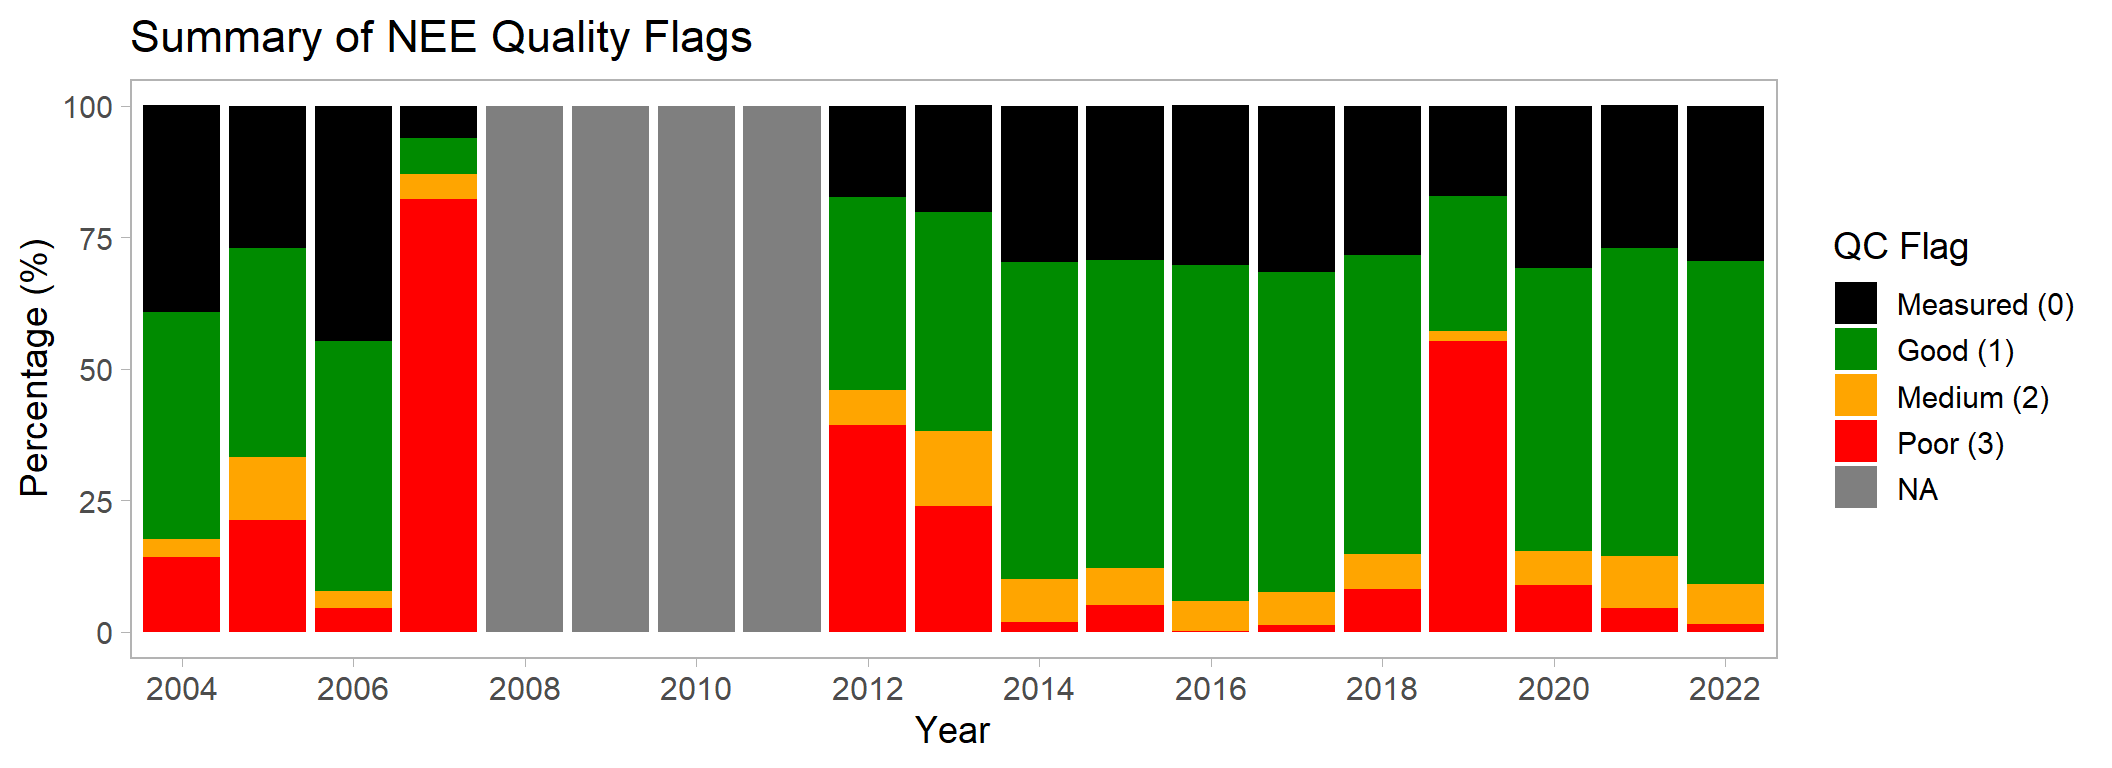
\includegraphics{FLUXNET_files/figure-latex/unnamed-chunk-8-1.pdf}

\begin{Shaded}
\begin{Highlighting}[]
\NormalTok{qc\_labels }\OtherTok{\textless{}{-}}\NormalTok{ qc\_summary }\SpecialCharTok{\%\textgreater{}\%}
  \FunctionTok{group\_by}\NormalTok{(year) }\SpecialCharTok{\%\textgreater{}\%}
  \FunctionTok{summarise}\NormalTok{(}
    \AttributeTok{qc\_text =} \FunctionTok{paste}\NormalTok{(label, }\AttributeTok{collapse =} \StringTok{"}\SpecialCharTok{\textbackslash{}n}\StringTok{"}\NormalTok{),}
    \AttributeTok{.groups =} \StringTok{"drop"}
\NormalTok{  )}

\NormalTok{data\_with\_labels }\OtherTok{\textless{}{-}}\NormalTok{ df.HH }\SpecialCharTok{\%\textgreater{}\%}
  \FunctionTok{left\_join}\NormalTok{(qc\_labels, }\AttributeTok{by =} \StringTok{"year"}\NormalTok{)}

\CommentTok{\# looking into data for one year: plot NEE with QC flags}
\NormalTok{data\_with\_labels }\SpecialCharTok{\%\textgreater{}\%}
  \FunctionTok{filter}\NormalTok{(year }\SpecialCharTok{==} \DecValTok{2018}\NormalTok{) }\SpecialCharTok{\%\textgreater{}\%} 
  \FunctionTok{ggplot}\NormalTok{(}\FunctionTok{aes}\NormalTok{(}\AttributeTok{x =}\NormalTok{ DOY, }\AttributeTok{y =}\NormalTok{ NEE\_VUT\_REF, }\AttributeTok{color =}\NormalTok{ qc\_label)) }\SpecialCharTok{+}
  \FunctionTok{geom\_point}\NormalTok{(}\AttributeTok{alpha =} \FloatTok{0.6}\NormalTok{, }\AttributeTok{size =} \DecValTok{1}\NormalTok{) }\SpecialCharTok{+}
  \FunctionTok{scale\_color\_manual}\NormalTok{(}
    \AttributeTok{name =} \StringTok{"QC Flag"}\NormalTok{,}
    \AttributeTok{values =} \FunctionTok{c}\NormalTok{(}\StringTok{"Measured (0)"} \OtherTok{=} \StringTok{"black"}\NormalTok{,}
               \StringTok{"Good (1)"} \OtherTok{=} \StringTok{"green4"}\NormalTok{,}
               \StringTok{"Medium (2)"} \OtherTok{=} \StringTok{"orange"}\NormalTok{,}
               \StringTok{"Poor (3)"} \OtherTok{=} \StringTok{"red"}\NormalTok{)}
\NormalTok{  ) }\SpecialCharTok{+}
  \FunctionTok{geom\_text}\NormalTok{(}
    \AttributeTok{data =}\NormalTok{ qc\_labels,}
    \FunctionTok{aes}\NormalTok{(}\AttributeTok{x =} \DecValTok{12}\NormalTok{, }\AttributeTok{y =} \DecValTok{20}\NormalTok{, }\AttributeTok{label =}\NormalTok{ qc\_text),}
    \AttributeTok{inherit.aes =} \ConstantTok{FALSE}\NormalTok{,}
    \AttributeTok{hjust =} \DecValTok{0}\NormalTok{,}
    \AttributeTok{vjust =} \FloatTok{1.1}\NormalTok{,}
    \AttributeTok{size =} \DecValTok{3}\NormalTok{,}
    \AttributeTok{color =} \StringTok{"gray30"}
\NormalTok{  ) }\SpecialCharTok{+}
  \FunctionTok{labs}\NormalTok{(}
    \AttributeTok{title =} \StringTok{"Half hourly FCO2 and quality flags for a single year"}\NormalTok{,}
    \AttributeTok{x =} \StringTok{"DOY"}\NormalTok{, }\AttributeTok{y =} \FunctionTok{expression}\NormalTok{(FCO2}\SpecialCharTok{\textasciitilde{}}\NormalTok{(g}\SpecialCharTok{\textasciitilde{}}\NormalTok{C}\SpecialCharTok{\textasciitilde{}}\NormalTok{m}\SpecialCharTok{\^{}}\NormalTok{\{}\SpecialCharTok{{-}}\DecValTok{2}\NormalTok{\}}\SpecialCharTok{\textasciitilde{}}\NormalTok{d}\SpecialCharTok{\^{}}\NormalTok{\{}\SpecialCharTok{{-}}\DecValTok{1}\NormalTok{\})) }
\NormalTok{  ) }\SpecialCharTok{+}\NormalTok{ my\_theme}
\end{Highlighting}
\end{Shaded}

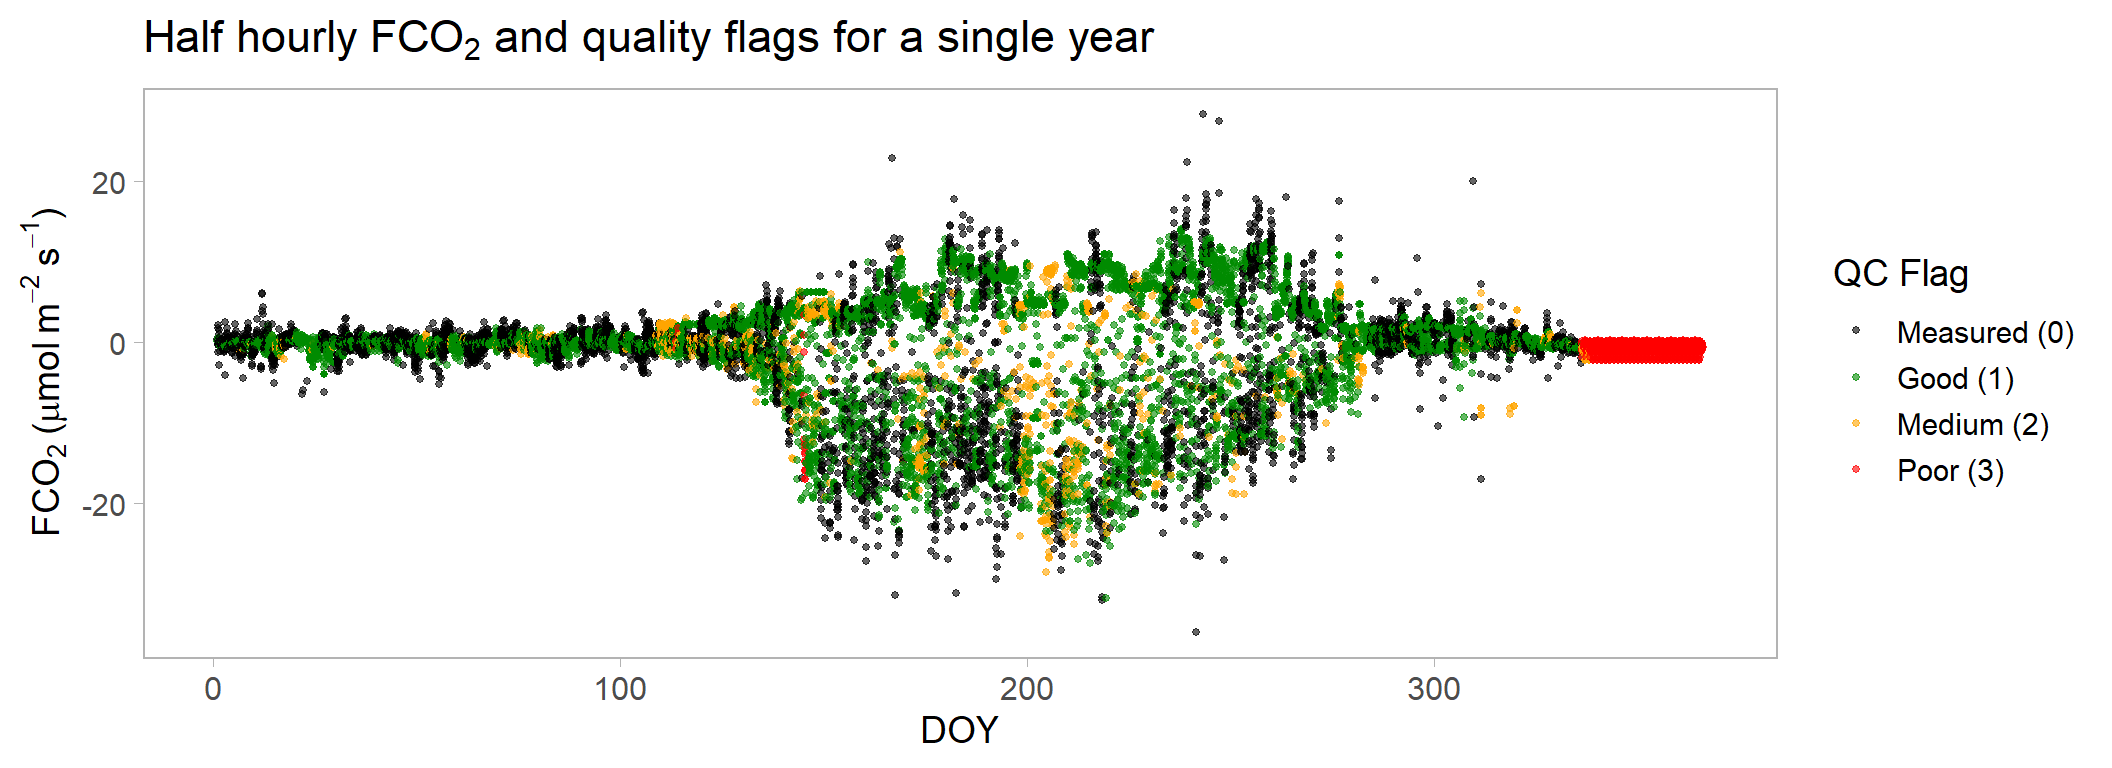
\includegraphics{FLUXNET_files/figure-latex/unnamed-chunk-8-2.pdf} Where
to go from here: - Interpret the figure and include it in your group
presentation.

\section{Optional: Ecosystem water
budget}\label{optional-ecosystem-water-budget}

ET = Evapotranspiration = the sum of evaporation from soil +
transpiration from plants. P = Precipitation = all water input from
rain/snow.

\begin{Shaded}
\begin{Highlighting}[]
\CommentTok{\# https://rdrr.io/cran/bigleaf/man/LE.to.ET.html}
\NormalTok{monthly\_data }\OtherTok{\textless{}{-}}\NormalTok{ monthly\_data }\SpecialCharTok{\%\textgreater{}\%}
  \FunctionTok{mutate}\NormalTok{(}\AttributeTok{y\_label\_pos =} \FunctionTok{max}\NormalTok{(P, ET, }\AttributeTok{na.rm =} \ConstantTok{TRUE}\NormalTok{) }\SpecialCharTok{*} \DecValTok{1}\NormalTok{)}

\CommentTok{\# Add ET/P ratio to monthly\_data}
\NormalTok{monthly\_data }\OtherTok{\textless{}{-}}\NormalTok{ monthly\_data }\SpecialCharTok{\%\textgreater{}\%}
  \FunctionTok{mutate}\NormalTok{(}\AttributeTok{ET\_P\_ratio =}\NormalTok{ ET }\SpecialCharTok{/}\NormalTok{ P)}

\CommentTok{\# Add GPP/ET ratio to monthly\_data for WUE}
\NormalTok{monthly\_data }\OtherTok{\textless{}{-}}\NormalTok{ monthly\_data }\SpecialCharTok{\%\textgreater{}\%}
  \FunctionTok{mutate}\NormalTok{(}\AttributeTok{WUE =} \SpecialCharTok{{-}}\NormalTok{(GPP)}\SpecialCharTok{/}\NormalTok{ET)}

\CommentTok{\# monthly\_data \textless{}{-} monthly\_data \%\textgreater{}\%}
\CommentTok{\#   mutate(y\_label\_pos = max(P, ET, na.rm = TRUE) * 1)}

\CommentTok{\# plot: P and ET}
\FunctionTok{ggplot}\NormalTok{(monthly\_data, }\FunctionTok{aes}\NormalTok{(}\AttributeTok{x =}\NormalTok{ month\_year)) }\SpecialCharTok{+}
  \FunctionTok{geom\_bar}\NormalTok{(}\FunctionTok{aes}\NormalTok{(}\AttributeTok{y =}\NormalTok{ P, }\AttributeTok{fill =} \StringTok{"P"}\NormalTok{), }\AttributeTok{stat =} \StringTok{"identity"}\NormalTok{, }\AttributeTok{position =} \StringTok{"dodge"}\NormalTok{, }\AttributeTok{alpha =} \FloatTok{0.7}\NormalTok{) }\SpecialCharTok{+}
  \FunctionTok{geom\_line}\NormalTok{(}\FunctionTok{aes}\NormalTok{(}\AttributeTok{y =}\NormalTok{ ET, }\AttributeTok{color =} \StringTok{"ET"}\NormalTok{), }\AttributeTok{size =} \DecValTok{1}\NormalTok{) }\SpecialCharTok{+}
  \FunctionTok{geom\_vline}\NormalTok{(}\AttributeTok{data =}\NormalTok{ monthly\_data }\SpecialCharTok{\%\textgreater{}\%} \FunctionTok{filter}\NormalTok{(month }\SpecialCharTok{==} \DecValTok{12}\NormalTok{), }
             \FunctionTok{aes}\NormalTok{(}\AttributeTok{xintercept =} \FunctionTok{as.numeric}\NormalTok{(month\_year) }\SpecialCharTok{+} \DecValTok{15}\NormalTok{), }
             \AttributeTok{linetype =} \StringTok{"dashed"}\NormalTok{, }\AttributeTok{color =} \StringTok{"black"}\NormalTok{, }\AttributeTok{size =} \FloatTok{0.5}\NormalTok{) }\SpecialCharTok{+}
  \FunctionTok{geom\_text}\NormalTok{(}\AttributeTok{data =}\NormalTok{ monthly\_data }\SpecialCharTok{\%\textgreater{}\%} \FunctionTok{filter}\NormalTok{(month }\SpecialCharTok{==} \DecValTok{6}\NormalTok{), }
            \FunctionTok{aes}\NormalTok{(}\AttributeTok{x =}\NormalTok{ year\_label\_pos, }
                \AttributeTok{y =} \FunctionTok{max}\NormalTok{(ET, P, }\AttributeTok{na.rm =} \ConstantTok{TRUE}\NormalTok{) }\SpecialCharTok{*} \DecValTok{1}\NormalTok{,  }\CommentTok{\# Adjust label position based on max value}
                \AttributeTok{label =}\NormalTok{ year), }
            \AttributeTok{color =} \StringTok{"black"}\NormalTok{, }\AttributeTok{size =} \DecValTok{5}\NormalTok{, }\AttributeTok{fontface =} \StringTok{"bold"}\NormalTok{) }\SpecialCharTok{+}
  \FunctionTok{labs}\NormalTok{(}\AttributeTok{x =} \StringTok{"Month"}\NormalTok{, }\AttributeTok{y =} \FunctionTok{expression}\NormalTok{(}\StringTok{"mm of water"}\NormalTok{), }\AttributeTok{title =} \StringTok{"Monthly ET and P Trends"}\NormalTok{) }\SpecialCharTok{+}
  \FunctionTok{scale\_fill\_manual}\NormalTok{(}\AttributeTok{values =} \FunctionTok{c}\NormalTok{(}\StringTok{"P"} \OtherTok{=} \StringTok{"gray"}\NormalTok{)) }\SpecialCharTok{+}  \CommentTok{\# P (bars)}
  \FunctionTok{scale\_color\_manual}\NormalTok{(}\AttributeTok{values =} \FunctionTok{c}\NormalTok{(}\StringTok{"ET"} \OtherTok{=} \StringTok{"\#F8766D"}\NormalTok{)) }\SpecialCharTok{+}  \CommentTok{\# ET (line)}
  \FunctionTok{scale\_x\_date}\NormalTok{(}\AttributeTok{date\_labels =} \StringTok{"\%m"}\NormalTok{, }\AttributeTok{date\_breaks =} \StringTok{"6 month"}\NormalTok{, }\AttributeTok{expand =} \FunctionTok{c}\NormalTok{(}\DecValTok{0}\NormalTok{, }\DecValTok{0}\NormalTok{)) }\SpecialCharTok{+}  
  \FunctionTok{scale\_y\_continuous}\NormalTok{(}
    \AttributeTok{breaks =} \FunctionTok{seq}\NormalTok{(}\DecValTok{0}\NormalTok{, }\FunctionTok{ceiling}\NormalTok{(}\FunctionTok{max}\NormalTok{(monthly\_data}\SpecialCharTok{$}\NormalTok{ET, monthly\_data}\SpecialCharTok{$}\NormalTok{P, }\AttributeTok{na.rm =} \ConstantTok{TRUE}\NormalTok{) }\SpecialCharTok{+} \DecValTok{5}\NormalTok{), }\AttributeTok{by =} \DecValTok{50}\NormalTok{),}
    \AttributeTok{limits =} \FunctionTok{c}\NormalTok{(}\DecValTok{0}\NormalTok{, }\FunctionTok{ceiling}\NormalTok{(}\FunctionTok{max}\NormalTok{(monthly\_data}\SpecialCharTok{$}\NormalTok{ET, monthly\_data}\SpecialCharTok{$}\NormalTok{P, }\AttributeTok{na.rm =} \ConstantTok{TRUE}\NormalTok{) }\SpecialCharTok{+} \DecValTok{5}\NormalTok{))}
\NormalTok{  )  }\SpecialCharTok{+}\NormalTok{ my\_theme}
\end{Highlighting}
\end{Shaded}

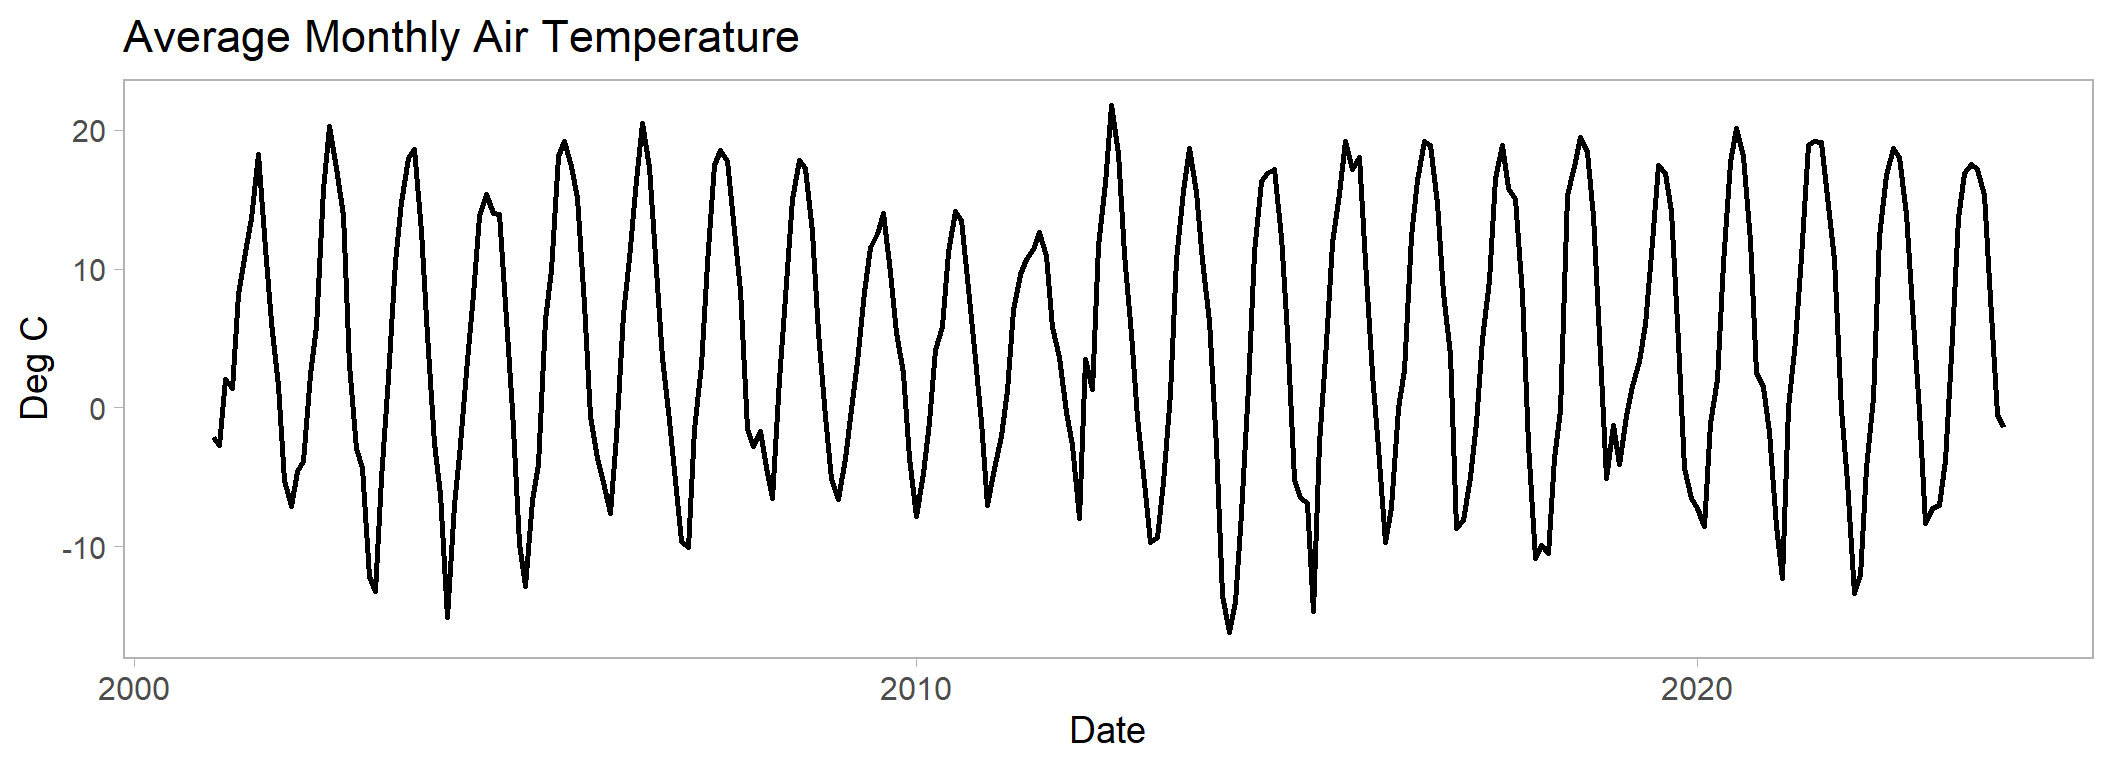
\includegraphics{FLUXNET_files/figure-latex/unnamed-chunk-9-1.pdf}

\begin{Shaded}
\begin{Highlighting}[]
\CommentTok{\# plot: water use efficiency}
\FunctionTok{ggplot}\NormalTok{(monthly\_data, }\FunctionTok{aes}\NormalTok{(}\AttributeTok{x =}\NormalTok{ month\_year, }\AttributeTok{y =}\NormalTok{ WUE)) }\SpecialCharTok{+}
  \FunctionTok{geom\_bar}\NormalTok{(}\AttributeTok{stat =} \StringTok{"identity"}\NormalTok{, }\AttributeTok{fill =} \StringTok{"\#619CFF"}\NormalTok{, }\AttributeTok{alpha =} \FloatTok{0.8}\NormalTok{) }\SpecialCharTok{+}
  \FunctionTok{labs}\NormalTok{(}\AttributeTok{x =} \StringTok{"Month"}\NormalTok{, }\AttributeTok{y =} \StringTok{"WUE"}\NormalTok{, }\AttributeTok{title =} \StringTok{"Water{-}use efficiency (GPP/ET)"}\NormalTok{) }\SpecialCharTok{+}
  \FunctionTok{geom\_vline}\NormalTok{(}\AttributeTok{data =}\NormalTok{ monthly\_data }\SpecialCharTok{\%\textgreater{}\%} \FunctionTok{filter}\NormalTok{(month }\SpecialCharTok{==} \DecValTok{12}\NormalTok{), }
             \FunctionTok{aes}\NormalTok{(}\AttributeTok{xintercept =} \FunctionTok{as.numeric}\NormalTok{(month\_year) }\SpecialCharTok{+} \DecValTok{15}\NormalTok{), }
             \AttributeTok{linetype =} \StringTok{"dashed"}\NormalTok{, }\AttributeTok{color =} \StringTok{"black"}\NormalTok{, }\AttributeTok{size =} \FloatTok{0.5}\NormalTok{) }\SpecialCharTok{+}
  \FunctionTok{geom\_hline}\NormalTok{(}\AttributeTok{yintercept =} \DecValTok{1}\NormalTok{, }\AttributeTok{linetype =} \StringTok{"dashed"}\NormalTok{, }\AttributeTok{color =} \StringTok{"black"}\NormalTok{, }\AttributeTok{size =} \FloatTok{0.8}\NormalTok{) }\SpecialCharTok{+}
  \FunctionTok{geom\_text}\NormalTok{(}\AttributeTok{data =}\NormalTok{ monthly\_data }\SpecialCharTok{\%\textgreater{}\%} \FunctionTok{filter}\NormalTok{(month }\SpecialCharTok{==} \DecValTok{6}\NormalTok{), }
            \FunctionTok{aes}\NormalTok{(}\AttributeTok{x =}\NormalTok{ year\_label\_pos, }
                \AttributeTok{y =} \DecValTok{60}\NormalTok{,  }\CommentTok{\# Adjust label position based on max value}
                \AttributeTok{label =}\NormalTok{ year), }
            \AttributeTok{color =} \StringTok{"black"}\NormalTok{, }\AttributeTok{size =} \DecValTok{5}\NormalTok{, }\AttributeTok{fontface =} \StringTok{"bold"}\NormalTok{) }\SpecialCharTok{+}
  \FunctionTok{scale\_x\_date}\NormalTok{(}\AttributeTok{date\_labels =} \StringTok{"\%m"}\NormalTok{, }\AttributeTok{date\_breaks =} \StringTok{"6 month"}\NormalTok{, }\AttributeTok{expand =} \FunctionTok{c}\NormalTok{(}\DecValTok{0}\NormalTok{, }\DecValTok{0}\NormalTok{)) }\SpecialCharTok{+}
  \FunctionTok{scale\_y\_continuous}\NormalTok{(}
    \AttributeTok{breaks =} \FunctionTok{seq}\NormalTok{(}\DecValTok{0}\NormalTok{, }\FunctionTok{ceiling}\NormalTok{(}\FunctionTok{max}\NormalTok{(monthly\_data}\SpecialCharTok{$}\NormalTok{WUE, }\AttributeTok{na.rm =} \ConstantTok{TRUE}\NormalTok{) }\SpecialCharTok{+} \DecValTok{1}\NormalTok{), }\AttributeTok{by =} \DecValTok{10}\NormalTok{),}
    \AttributeTok{limits =} \FunctionTok{c}\NormalTok{(}\DecValTok{0}\NormalTok{, }\FunctionTok{ceiling}\NormalTok{(}\FunctionTok{max}\NormalTok{(monthly\_data}\SpecialCharTok{$}\NormalTok{WUE, }\AttributeTok{na.rm =} \ConstantTok{TRUE}\NormalTok{) }\SpecialCharTok{+} \FloatTok{0.5}\NormalTok{))}
\NormalTok{  ) }\SpecialCharTok{+}\NormalTok{ my\_theme}
\end{Highlighting}
\end{Shaded}

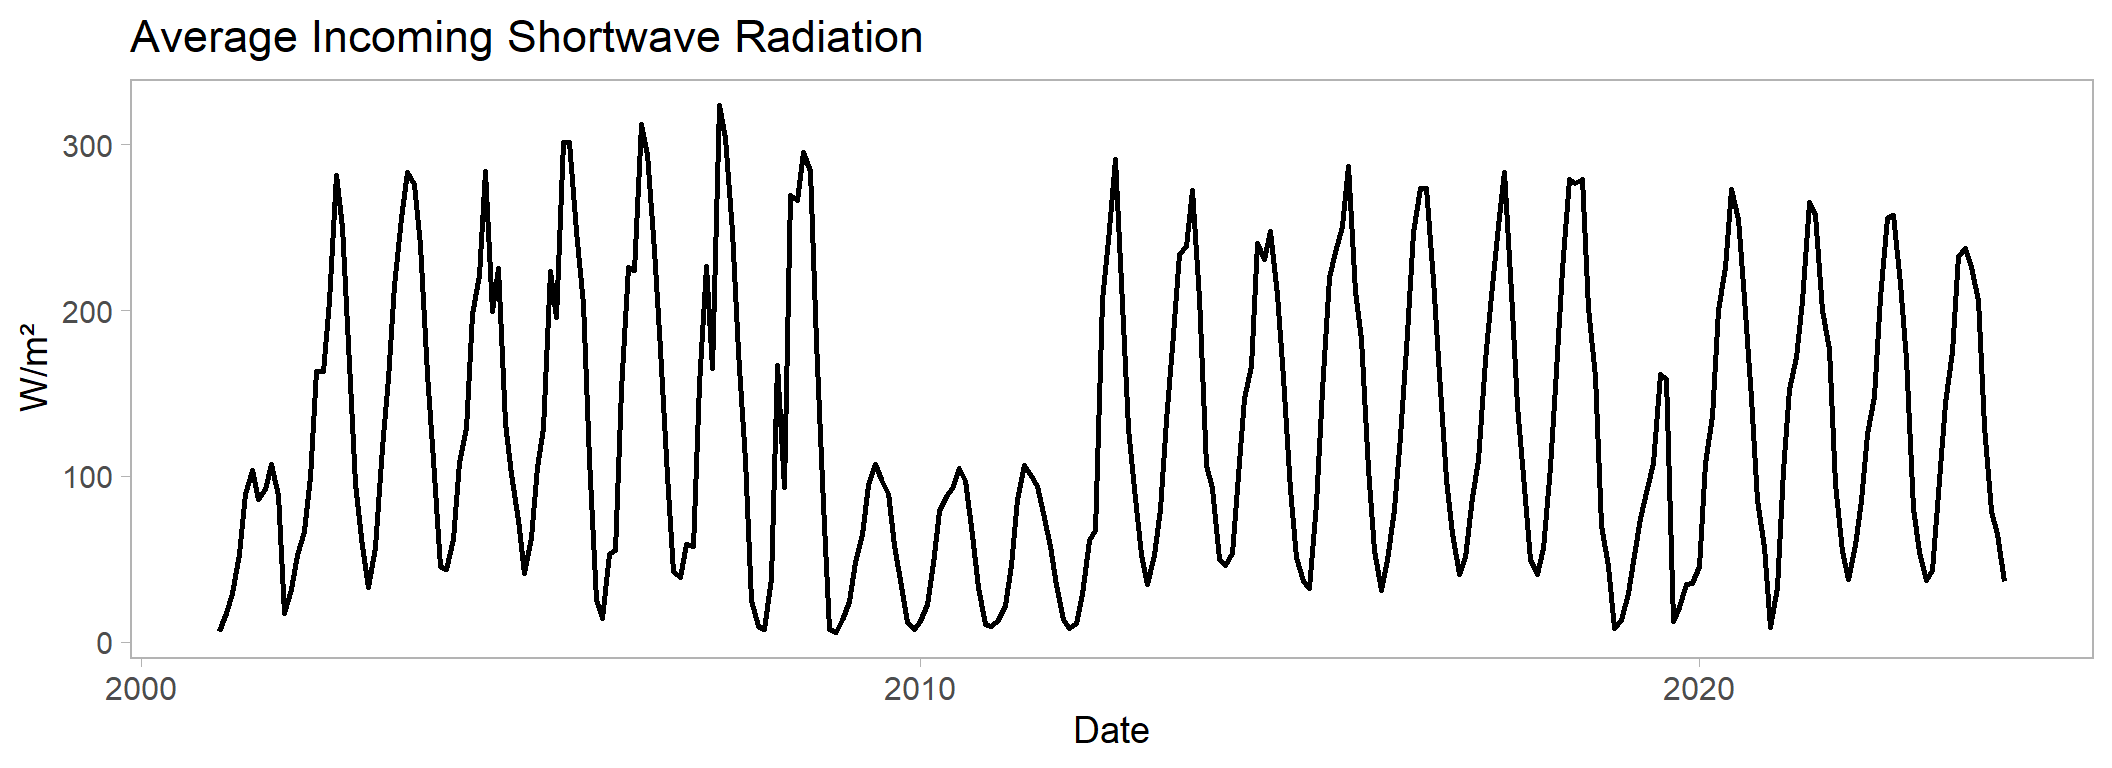
\includegraphics{FLUXNET_files/figure-latex/unnamed-chunk-9-2.pdf}

\begin{Shaded}
\begin{Highlighting}[]
\CommentTok{\# For winter, snowfall melt is }
\CommentTok{\# WUE: only for growing season: focus on peak growing season only ... why }
\end{Highlighting}
\end{Shaded}

Where to go from here: - Interpret the figure and include it in your
group presentation.

\section{Optional: Light use
efficiency}\label{optional-light-use-efficiency}

\begin{Shaded}
\begin{Highlighting}[]
\NormalTok{data\_filtered }\OtherTok{=}\NormalTok{ df.HH[df.HH}\SpecialCharTok{$}\NormalTok{month }\SpecialCharTok{==} \DecValTok{7}\NormalTok{, ] }\CommentTok{\# specify the period you want like to focus on}
\NormalTok{data\_filtered}\SpecialCharTok{$}\NormalTok{PPFD }\OtherTok{=}\NormalTok{ data\_filtered}\SpecialCharTok{$}\NormalTok{PPFD\_IN}
\NormalTok{data\_filtered}\SpecialCharTok{$}\NormalTok{NEE }\OtherTok{=}\NormalTok{ data\_filtered}\SpecialCharTok{$}\NormalTok{NEE\_VUT\_REF}

\CommentTok{\# Function to calculate light response curve for NEE based on the Michaelis{-}Menten equation}
\NormalTok{light\_response\_NEE }\OtherTok{\textless{}{-}} \ControlFlowTok{function}\NormalTok{(PPFD, Amax, alpha, Rd) \{}
  \SpecialCharTok{{-}}\NormalTok{((Amax }\SpecialCharTok{*}\NormalTok{ PPFD) }\SpecialCharTok{/}\NormalTok{ (alpha }\SpecialCharTok{+}\NormalTok{ PPFD) }\SpecialCharTok{{-}}\NormalTok{ Rd)}
\NormalTok{\}}

\NormalTok{fit\_NEE }\OtherTok{\textless{}{-}} \FunctionTok{nls}\NormalTok{(NEE }\SpecialCharTok{\textasciitilde{}} \FunctionTok{light\_response\_NEE}\NormalTok{(PPFD, Amax, alpha, Rd),}
               \AttributeTok{data =}\NormalTok{ data\_filtered,}
               \AttributeTok{start =} \FunctionTok{list}\NormalTok{(}\AttributeTok{Amax =} \FunctionTok{max}\NormalTok{(}\SpecialCharTok{{-}}\NormalTok{data\_filtered}\SpecialCharTok{$}\NormalTok{NEE, }\AttributeTok{na.rm =} \ConstantTok{TRUE}\NormalTok{),}
                            \AttributeTok{alpha =} \DecValTok{200}\NormalTok{, }\AttributeTok{Rd =} \DecValTok{2}\NormalTok{))}

\CommentTok{\# Extract model parameter estimates}
\NormalTok{params }\OtherTok{\textless{}{-}} \FunctionTok{coef}\NormalTok{(fit\_NEE)}
\NormalTok{Amax\_est }\OtherTok{\textless{}{-}} \FunctionTok{round}\NormalTok{(params[}\StringTok{"Amax"}\NormalTok{], }\DecValTok{2}\NormalTok{)}
\NormalTok{alpha\_est }\OtherTok{\textless{}{-}} \FunctionTok{round}\NormalTok{(params[}\StringTok{"alpha"}\NormalTok{], }\DecValTok{2}\NormalTok{)}
\NormalTok{Rd\_est }\OtherTok{\textless{}{-}} \FunctionTok{round}\NormalTok{(params[}\StringTok{"Rd"}\NormalTok{], }\DecValTok{2}\NormalTok{)}
\CommentTok{\# compute A2000}
\NormalTok{A2000 }\OtherTok{=}\NormalTok{ Amax\_est }\SpecialCharTok{*} \DecValTok{2000}\SpecialCharTok{/}\NormalTok{(alpha\_est }\SpecialCharTok{+} \DecValTok{2000}\NormalTok{)}

\CommentTok{\# Generate predicted values from the fitted model}
\NormalTok{data\_filtered}\SpecialCharTok{$}\NormalTok{NEE\_pred }\OtherTok{\textless{}{-}} \FunctionTok{predict}\NormalTok{(fit\_NEE, }\AttributeTok{newdata =}\NormalTok{ data\_filtered)}
\FunctionTok{ggplot}\NormalTok{(data\_filtered, }\FunctionTok{aes}\NormalTok{(}\AttributeTok{x =}\NormalTok{ PPFD, }\AttributeTok{y =}\NormalTok{ NEE))  }\SpecialCharTok{+}
  \FunctionTok{geom\_point}\NormalTok{() }\SpecialCharTok{+}
  \FunctionTok{geom\_line}\NormalTok{(}\FunctionTok{aes}\NormalTok{(}\AttributeTok{y =}\NormalTok{ NEE\_pred), }\AttributeTok{color =} \StringTok{"red"}\NormalTok{, }\AttributeTok{size =} \FloatTok{1.2}\NormalTok{) }\SpecialCharTok{+}  
  \FunctionTok{geom\_hline}\NormalTok{(}\AttributeTok{yintercept =} \DecValTok{0}\NormalTok{, }\AttributeTok{linetype =} \StringTok{"dashed"}\NormalTok{, }\AttributeTok{color =} \StringTok{"grey"}\NormalTok{, }\AttributeTok{size =} \DecValTok{1}\NormalTok{) }\SpecialCharTok{+}  
  \FunctionTok{geom\_vline}\NormalTok{(}\AttributeTok{xintercept =} \DecValTok{1800}\NormalTok{, }\AttributeTok{linetype =} \StringTok{"dashed"}\NormalTok{, }\AttributeTok{color =} \StringTok{"grey"}\NormalTok{, }\AttributeTok{size =} \DecValTok{1}\NormalTok{) }\SpecialCharTok{+}
  \FunctionTok{labs}\NormalTok{(}\AttributeTok{x =} \FunctionTok{expression}\NormalTok{(PPFD }\SpecialCharTok{\textasciitilde{}} \StringTok{"("} \SpecialCharTok{*}\NormalTok{ mu }\SpecialCharTok{*} \StringTok{"mol"} \SpecialCharTok{\textasciitilde{}}\NormalTok{ m}\SpecialCharTok{\^{}}\NormalTok{\{}\SpecialCharTok{{-}}\DecValTok{2}\NormalTok{\} }\SpecialCharTok{\textasciitilde{}}\NormalTok{ s}\SpecialCharTok{\^{}}\NormalTok{\{}\SpecialCharTok{{-}}\DecValTok{1}\NormalTok{\} }\SpecialCharTok{*} \StringTok{")"}\NormalTok{), }
       \AttributeTok{y =} \FunctionTok{expression}\NormalTok{(FCO[}\DecValTok{2}\NormalTok{] }\SpecialCharTok{\textasciitilde{}} \StringTok{"("} \SpecialCharTok{*}\NormalTok{ mu }\SpecialCharTok{*} \StringTok{"mol"} \SpecialCharTok{\textasciitilde{}}\NormalTok{ m}\SpecialCharTok{\^{}}\NormalTok{\{}\SpecialCharTok{{-}}\DecValTok{2}\NormalTok{\} }\SpecialCharTok{\textasciitilde{}}\NormalTok{ s}\SpecialCharTok{\^{}}\NormalTok{\{}\SpecialCharTok{{-}}\DecValTok{1}\NormalTok{\} }\SpecialCharTok{*} \StringTok{")"}\NormalTok{)) }\SpecialCharTok{+}
\NormalTok{  my\_theme}
\end{Highlighting}
\end{Shaded}

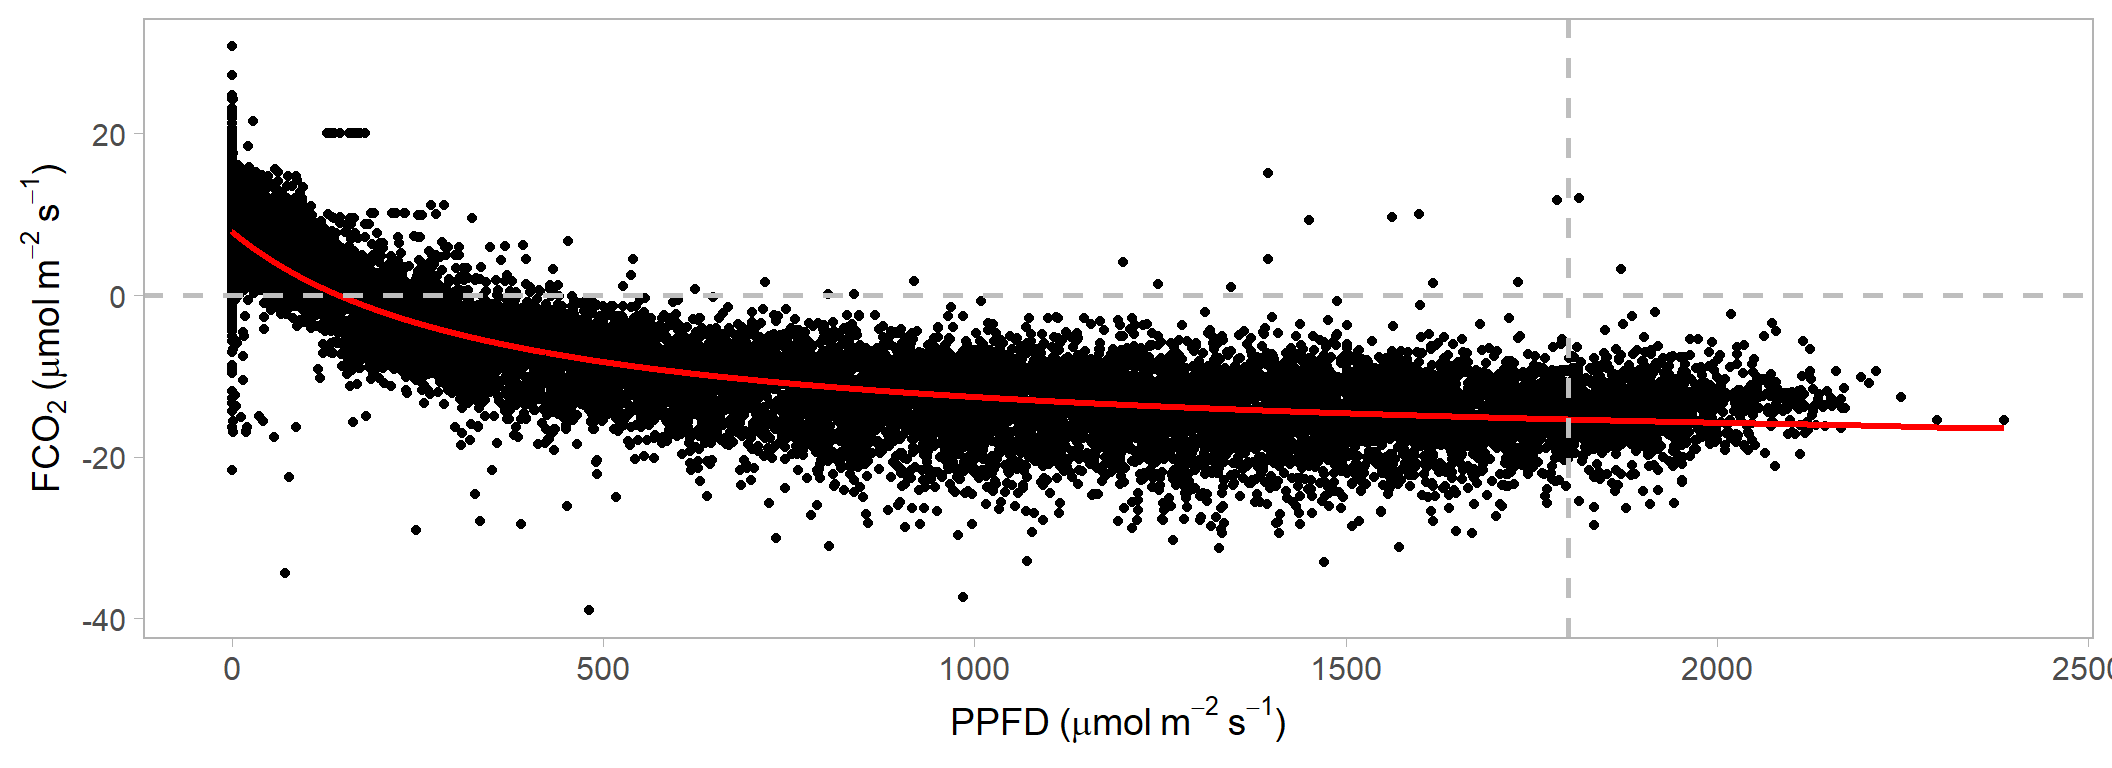
\includegraphics{FLUXNET_files/figure-latex/unnamed-chunk-10-1.pdf}

\begin{Shaded}
\begin{Highlighting}[]
\CommentTok{\# Function to compute A2000  }
\NormalTok{fit\_light\_response\_NEE }\OtherTok{\textless{}{-}} \ControlFlowTok{function}\NormalTok{(data) \{}
  \CommentTok{\# Skip if not enough data}
  \ControlFlowTok{if}\NormalTok{ (}\FunctionTok{nrow}\NormalTok{(data) }\SpecialCharTok{\textless{}} \DecValTok{10} \SpecialCharTok{||} \FunctionTok{all}\NormalTok{(}\FunctionTok{is.na}\NormalTok{(data}\SpecialCharTok{$}\NormalTok{NEE))) }\FunctionTok{return}\NormalTok{(}\ConstantTok{NULL}\NormalTok{)}

  \CommentTok{\# Michaelis{-}Menten light response model}
\NormalTok{  light\_response\_NEE }\OtherTok{\textless{}{-}} \ControlFlowTok{function}\NormalTok{(PPFD, Amax, alpha, Rd) \{}
    \SpecialCharTok{{-}}\NormalTok{((Amax }\SpecialCharTok{*}\NormalTok{ PPFD) }\SpecialCharTok{/}\NormalTok{ (alpha }\SpecialCharTok{+}\NormalTok{ PPFD) }\SpecialCharTok{{-}}\NormalTok{ Rd)}
\NormalTok{  \}}

  \CommentTok{\# Try fitting the model, catch failures}
\NormalTok{  fit\_result }\OtherTok{\textless{}{-}} \FunctionTok{tryCatch}\NormalTok{(\{}
    \FunctionTok{nls}\NormalTok{(NEE }\SpecialCharTok{\textasciitilde{}} \FunctionTok{light\_response\_NEE}\NormalTok{(PPFD, Amax, alpha, Rd),}
        \AttributeTok{data =}\NormalTok{ data,}
        \AttributeTok{start =} \FunctionTok{list}\NormalTok{(}
          \AttributeTok{Amax =} \FunctionTok{max}\NormalTok{(}\SpecialCharTok{{-}}\NormalTok{data}\SpecialCharTok{$}\NormalTok{NEE, }\AttributeTok{na.rm =} \ConstantTok{TRUE}\NormalTok{),  }\CommentTok{\# guess based on data}
          \AttributeTok{alpha =} \DecValTok{200}\NormalTok{,}
          \AttributeTok{Rd =} \DecValTok{2}
\NormalTok{        ),}
        \AttributeTok{control =} \FunctionTok{nls.control}\NormalTok{(}\AttributeTok{maxiter =} \DecValTok{100}\NormalTok{, }\AttributeTok{warnOnly =} \ConstantTok{TRUE}\NormalTok{)}
\NormalTok{    )}
\NormalTok{  \}, }\AttributeTok{error =} \ControlFlowTok{function}\NormalTok{(e) \{}
    \FunctionTok{message}\NormalTok{(}\StringTok{"Model failed for one year: "}\NormalTok{, e}\SpecialCharTok{$}\NormalTok{message)}
    \FunctionTok{return}\NormalTok{(}\ConstantTok{NULL}\NormalTok{)}
\NormalTok{  \})}

  \CommentTok{\# If fitting was successful, extract A2000}
  \ControlFlowTok{if}\NormalTok{ (}\SpecialCharTok{!}\FunctionTok{is.null}\NormalTok{(fit\_result)) \{}
\NormalTok{    params }\OtherTok{\textless{}{-}} \FunctionTok{coef}\NormalTok{(fit\_result)}
\NormalTok{    Amax }\OtherTok{\textless{}{-}}\NormalTok{ params[}\StringTok{"Amax"}\NormalTok{]}
\NormalTok{    alpha }\OtherTok{\textless{}{-}}\NormalTok{ params[}\StringTok{"alpha"}\NormalTok{]}
\NormalTok{    A2000 }\OtherTok{\textless{}{-}}\NormalTok{ Amax }\SpecialCharTok{*} \DecValTok{2000} \SpecialCharTok{/}\NormalTok{ (alpha }\SpecialCharTok{+} \DecValTok{2000}\NormalTok{)}
    \FunctionTok{return}\NormalTok{(}\FunctionTok{data.frame}\NormalTok{(}\AttributeTok{Amax =}\NormalTok{ Amax, }\AttributeTok{alpha =}\NormalTok{ alpha, }\AttributeTok{Rd =}\NormalTok{ params[}\StringTok{"Rd"}\NormalTok{], }\AttributeTok{A2000 =}\NormalTok{ A2000))}
\NormalTok{  \} }\ControlFlowTok{else}\NormalTok{ \{}
    \FunctionTok{return}\NormalTok{(}\ConstantTok{NULL}\NormalTok{)}
\NormalTok{  \}}
\NormalTok{\}}

\CommentTok{\# compute A2000 for each year}
\NormalTok{data\_by\_year }\OtherTok{\textless{}{-}} \FunctionTok{split}\NormalTok{(data\_filtered, data\_filtered}\SpecialCharTok{$}\NormalTok{year)}
\NormalTok{results\_by\_year }\OtherTok{\textless{}{-}} \FunctionTok{lapply}\NormalTok{(data\_by\_year, fit\_light\_response\_NEE)}
\FunctionTok{names}\NormalTok{(results\_by\_year) }\OtherTok{\textless{}{-}} \FunctionTok{names}\NormalTok{(data\_by\_year)}
\NormalTok{results\_df }\OtherTok{\textless{}{-}} \FunctionTok{bind\_rows}\NormalTok{(results\_by\_year, }\AttributeTok{.id =} \StringTok{"Year"}\NormalTok{)}

\FunctionTok{ggplot}\NormalTok{(results\_df, }\FunctionTok{aes}\NormalTok{(}\AttributeTok{x =} \FunctionTok{as.numeric}\NormalTok{(Year), }\AttributeTok{y =}\NormalTok{ A2000)) }\SpecialCharTok{+}
  \FunctionTok{geom\_line}\NormalTok{() }\SpecialCharTok{+}
  \FunctionTok{geom\_point}\NormalTok{() }\SpecialCharTok{+}
  \FunctionTok{labs}\NormalTok{(}\AttributeTok{title =} \StringTok{"A2000 over Years"}\NormalTok{, }\AttributeTok{x =} \StringTok{"Year"}\NormalTok{, }\AttributeTok{y =} \StringTok{"A2000 (µmol m⁻² s⁻¹)"}\NormalTok{) }\SpecialCharTok{+}
  \FunctionTok{ylim}\NormalTok{(}\DecValTok{0}\NormalTok{,}\DecValTok{50}\NormalTok{) }\SpecialCharTok{+}\NormalTok{ my\_theme}
\end{Highlighting}
\end{Shaded}

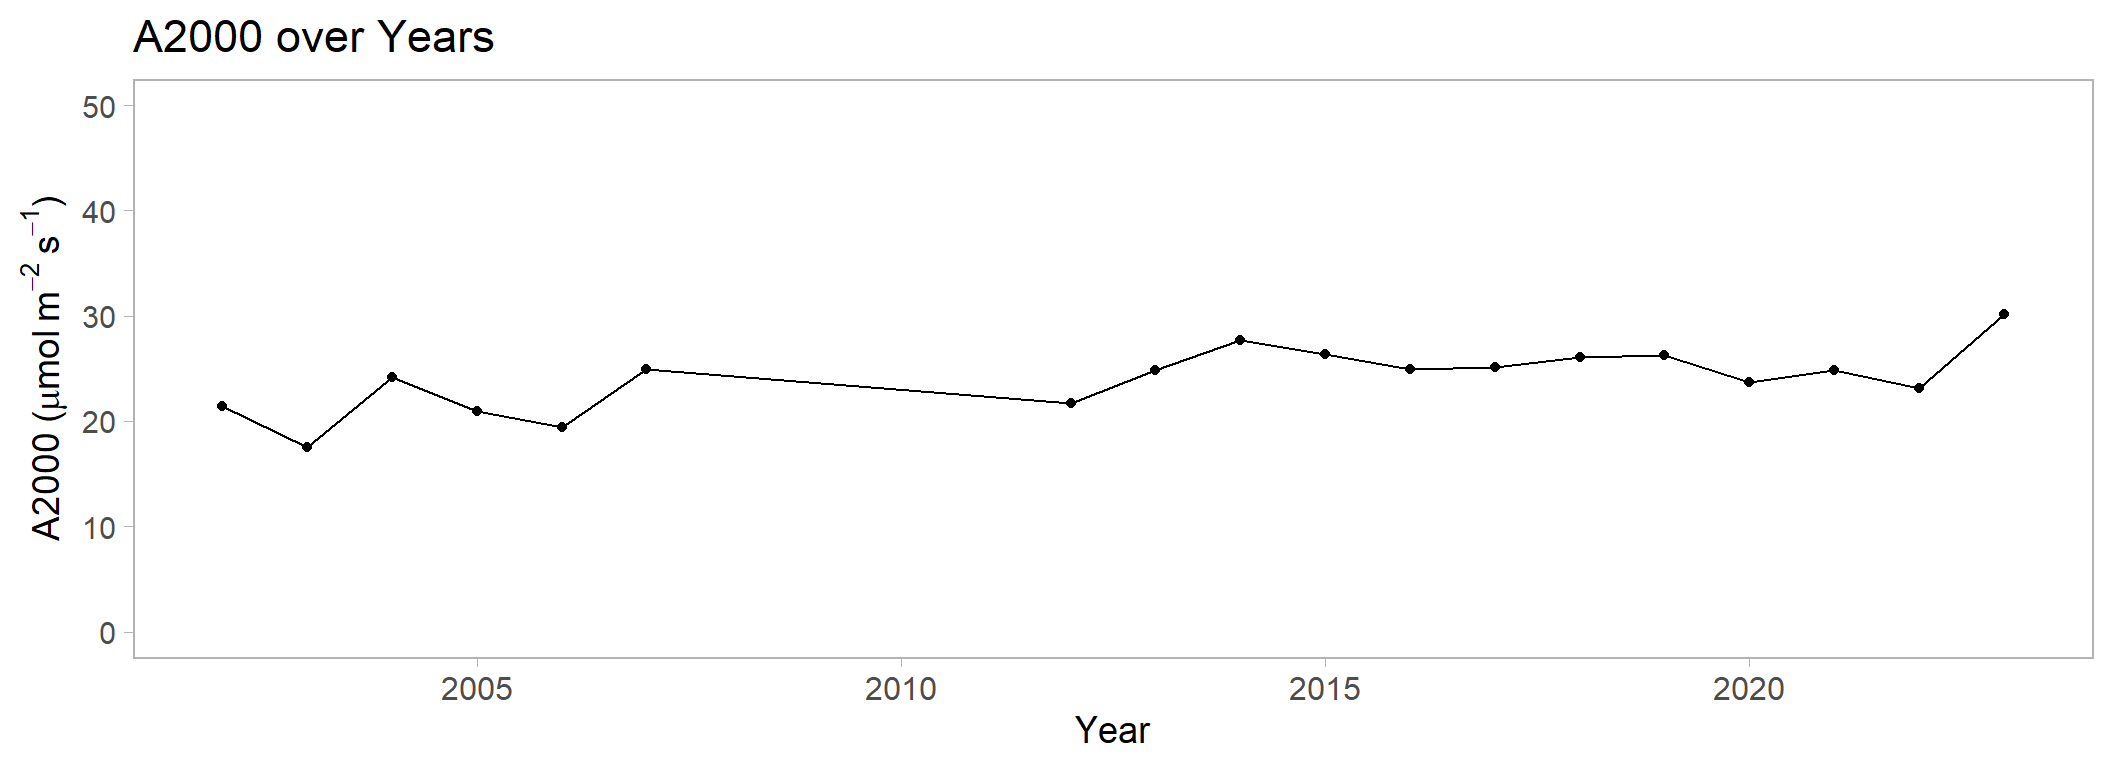
\includegraphics{FLUXNET_files/figure-latex/unnamed-chunk-10-2.pdf}
Where to go from here: - Interpret the figure and include it in your
group presentation. - Explore the seasonal pattern of A2000. - Group
discussion: What parameters used in land surface models relate to light
use and photosynthesis?

\section{Optional: Energy balance
closure}\label{optional-energy-balance-closure}

\begin{Shaded}
\begin{Highlighting}[]
\CommentTok{\# add some codes here}
\end{Highlighting}
\end{Shaded}

Where to go from here: - Interpret the figure and include it in your
group presentation. -

\section{Other ideas for group work:}\label{other-ideas-for-group-work}

\begin{itemize}
\tightlist
\item
  using \texttt{bigleaf} package to explore surface conductance and
  stomatal slope parameter;
  \url{https://cran.r-project.org/web/packages/bigleaf/vignettes/bigleaf_tutorial.pdf}
\end{itemize}

\section{References (MLA format)}\label{references-mla-format}

\begin{itemize}
\tightlist
\item
  Pastorello, Gilberto, et al.~``The FLUXNET2015 dataset and the ONEFlux
  processing pipeline for eddy covariance data.'' Scientific data 7.1
  (2020): 225.
\end{itemize}

\end{document}
